\Chapter{A fordítási probléma bemutatása}

A fejezet röviden bemutatja, hogy milyen koncepcionális problémák adódnak a célként kitűzött fordítási mechanizmus kapcsán. Röviden áttekinti továbbá a dolgozatban vizsgált megközelítéseket a fordító megvalósítására vonatkozóan.

\Section{Az objektum-relációs impedancia-eltérés}

A szoftverfejlesztés során az egyik leggyakrabban felmerülő architekturális kihívás az ob\-jek\-tum-relációs impedancia-eltérés (Object-Relational Impedance Mismatch) kezelése. Ez a jelenség abból fakad, hogy a relációs adatbázisok és az objektumorientált programozási nyelvek alapvetően eltérő paradigmákra épülnek. Míg az SQL alapú rendszerek adathalmazokban, táblákban és sorokban tárolják az információt, addig a C\# és más modern objektumorientált nyelvek objektumokban, valamint memóriabeli referenciagráfokban gondolkodnak \cite{skeet2019csharp}. 

Az SQL egy tisztán deklaratív nyelv, amely arra fókuszál, hogy \emph{mit} akarunk lekérdezni, a végrehajtás pontos lépéseinek definiálása nélkül. Bár a LINQ bevezeti a deklaratív adatelérés kényelmét a C\# nyelvbe, alapvetően mégis egy típusbiztos, imperatív ökoszisztémába ágyazódik be, ahol a lekérdezések láncolt metódushívásokra épülnek.

\Section{Az adatbázis-elérés megközelítései}

Az adatbázis-elérés különböző módszereit \aref{tab:adatbazis-eleres}. táblázat foglalja össze, az egyszerűbbtől a magasabb szintű absztrakció felé haladva.

\begin{table}[h]
	\centering
	\caption{Az adatbázis-elérés megközelítései}
	\label{tab:adatbazis-eleres}
	\renewcommand{\arraystretch}{1.4}
	\small
	\begin{tabular}{|p{0.19\textwidth}|p{0.28\textwidth}|p{0.37\textwidth}|}
		\hline
		\textbf{Megközelítés} & \textbf{Jellemző} & \textbf{Példa} \\
		\hline
		Nyers SQL string & Fordítási idejű ellenőrzés nélkül, SQL injekció veszélyével &
		\texttt{"SELECT * FROM Users} \newline \texttt{WHERE Id = " + id} \\
		\hline
		Paraméteres SQL & Biztonságos, de string alapú, sémaváltozásra érzékeny &
		\texttt{"SELECT * FROM Users} \newline \texttt{WHERE Id = @id"} \\
		\hline
		Micro-ORM (Dapper) & SQL stringek erős típusmegfeleltetéssel &
		\texttt{conn.Query<User>(} \newline \texttt{"SELECT ...",} \newline \texttt{new \{ Id = id \})} \\
		\hline
		LINQ + EF Core & Típusbiztos, fordítási idejű ellenőrzéssel, refaktorálható &
		\texttt{db.Users} \newline \texttt{.Where(x => x.Id == id)} \newline \texttt{.ToList()} \\
		\hline
	\end{tabular}
\end{table}

Ezen különbségek áthidalására a fejlesztők a múltban gyakran nyers SQL lekérdezéseket ágyaztak be az alkalmazás forráskódjába stringek formájában. Ez a megközelítés azonban komoly karbantarthatósági és biztonsági problémákkal járt. A beágyazott SQL stringek esetében a fordítóprogram (compiler) nem képes fordítási idejű (compile-time) szintaktikai vagy szemantikai ellenőrzést végezni. Ebből adódóan egy elgépelt oszlopnév vagy egy típusillesztési hiba kizárólag futásidőben (runtime) derül ki, ami jelentősen növeli a szoftver meghibásodásának kockázatát. Emellett az adatbázis-séma változásakor (például egy mező átnevezésekor) a modern integrált fejlesztőkörnyezetek (IDE) refaktoráló eszközei nem képesek automatikusan frissíteni a stringekben rejlő hivatkozásokat. Ezzel szemben a LINQ használatakor a típusos modelleken végzett módosítások a teljes lekérdezés-láncot automatikusan és biztonságosan frissítik \cite{skeet2019csharp}.

\Section{Az SQL és LINQ típusrendszerének kapcsolata}

A LINQ kétféle szintaxisban írható fel. Lekérdezési szintaxisban (\emph{query syntax}), amely az SQL-hez hasonló kulcsszavakat használ, és metódusszintaxisban (\emph{method syntax}), amely láncolt metódushívásokból áll. A fordító az utóbbit generálja. A lekérdezési szintaxis olvashatóbb ugyan egyszerű esetekben, de a kódgenerálás szempontjából lényeges hátránya, hogy a záradékok egy egységes blokkban jelennek meg, ahol az opcionális elemek elhagyása külön kezelést igényel. A metódusszintaxisnál ezzel szemben minden záradék önálló metódushívás, amelyet a generátor egyszerűen kihagyhat, ha az adott SQL utasításban nem szerepel. Ez a szerkezet közvetlen megfelelést teremt az AST csomópontjai és a generált lánc tagjai között, ami a kódgenerálást szabályosabbá és bővíthetőbbé teszi.

\begin{figure}[H]
	\centering
	\begin{tikzpicture}[
		node distance=0.6cm and 2.5cm,
		req/.style={draw, rounded corners=3pt, minimum width=2.8cm, minimum height=0.65cm, align=center, font=\small\ttfamily, fill=gray!20},
		opt/.style={draw, rounded corners=3pt, dashed, minimum width=2.8cm, minimum height=0.65cm, align=center, font=\small\ttfamily, fill=white},
		rep/.style={draw, rounded corners=3pt, minimum width=2.8cm, minimum height=0.65cm, align=center, font=\small\ttfamily, fill=gray!10},
		->,thick,>=stealth
		]
		
		\node[req] (from)    {db.Tabla};
		\node[rep, below=of from]    (join)    {.Join(...)};
		\node[rep, below=of join]    (where)   {.Where(...)};
		\node[opt, below=of where]   (groupby) {.GroupBy(...)};
		\node[opt, below=of groupby] (having)  {.Where(HAVING)};
		
		\node[req, right=of having]  (select)  {.Select(...)};
		\node[opt, above=of select]  (dist)    {.Distinct()};
		\node[opt, above=of dist]    (order)   {.OrderBy(...)};
		\node[opt, above=of order]   (take)    {.Take(n)};
		\node[opt, above=of take]    (skip)    {.Skip(n)};
		\node[req, above=of skip]    (exec)    {.ToList()};
		
		\draw (from)    -- (join);
		\draw (join)    -- (where);
		\draw (where)   -- (groupby);
		\draw (groupby) -- (having);
		\draw (having)  -- (select);
		\draw (select)  -- (dist);
		\draw (dist)    -- (order);
		\draw (order)   -- (take);
		\draw (take)    -- (skip);
		\draw (skip)    -- (exec);
		
		\draw[gray, densely dashed] (from.east) to[out=0,in=180] (select.west);
		\draw[gray, densely dashed] (where.west) to[out=180,in=180,looseness=2.5]
		node[left, font=\footnotesize\itshape]{*} (join.west);
		
	\end{tikzpicture}
	
	\vspace{0.5em}
	\small
	\begin{tabular}{@{}cll@{}}
		\tikz\node[draw, fill=gray!20, minimum width=0.6cm, minimum height=0.3cm, rounded corners=2pt, font=\tiny]{}; & kötelező & \\
		\tikz\node[draw, fill=gray!10, minimum width=0.6cm, minimum height=0.3cm, rounded corners=2pt, font=\tiny]{}; & ismételhető & \\
		\tikz\node[draw, dashed, minimum width=0.6cm, minimum height=0.3cm, rounded corners=2pt, font=\tiny]{}; & opcionális & \\
	\end{tabular}
	\caption{A LINQ metódusszintaxis lánc általános alakja}
\end{figure}

% TODO: Hivatkozni kellene az ábrát a szövegből.

% TODO: A Where-nél nem vagyok benne biztos, hogy ez így teljesen megfelelő. A Join és a Where sem biztos, hogy minden kifejezésben szerepel, illetve Where után is lehet Where.

\Section{A manuális átírás problémái}

Nagyobb méretű legacy rendszerek modernizálása során gyakori feladat a több ezer soros, elavult adatbázis-hívások átírása modern, Entity Framework Core alapú LINQ kifejezésekké. Ennek manuális elvégzése rendkívül időigényes, monoton és hibalehetőségekkel teli folyamat. A két nyelv szintaxisa és operátor-készlete közötti rejtett különbségek nehezen felderíthető logikai hibákhoz vezethetnek. Szemléletes példa lehet erre a logikai operátorok precedenciájának eltérése. Míg az SQL-ben a \texttt{NOT} operátor egyértelműen a teljes relációra vonatkoztatható anélkül, hogy típuskonfliktust okozna, addig a C\# \texttt{!} operátorának magasabb precedenciája miatt a kézi átírás során a megfelelő zárójelezés elhagyása azonnali fordítási hibát eredményezhet.

Ezen karbantartási és migrációs problémák kiküszöbölésére hatékony megoldást jelenthet egy transpiler megtervezése és alkalmazása. Egy ilyen eszköz létrehozása azonban specifikus technológiai kihívásokat is tartogat. Mivel a két nyelv nem feleltethető meg egymásnak egy az egyben, a fordítónak intelligens módon kell áthidalnia a hiányosságokat. Nem minden SQL utasításnak vagy beépített adatbázis függvénynek van közvetlen C\# megfelelője. Például az SQL \texttt{LIKE} operátorának és helyettesítő karaktereinek fordítására kézenfekvő megoldás lenne reguláris kifejezések generálása lenne, ez a megoldás azonban kliensoldali kiértékeléshez vezet. Továbbá a fordító által előállított LINQ kódnak nem csupán szintaktikailag kell helyesnek lennie, hanem illeszkednie kell az Entity Framework kifejezésfa (Expression Tree) kiértékelési mechanizmusaihoz is, elkerülve a nem támogatott szerveroldali fordításokat és a teljesítményt rontó kliensoldali adatfeldolgozást \cite{nmorph2023}.

A bemutatott fordító célja az SQL:1999 szabvány által definiált lekérdezésnyelv egy jól meghatározott részhalmazának lefordítása Entity Framework Core 8.0 kompatibilis LINQ metódusszintaxisra. A bemeneti nyelv az SQL:1999-es szabványt követi, a generált kimenet pedig olyan C\# kód, amely EF Core 8.0 alatt, bármely adatbázis-provider esetén szerver oldalon fordítható SQL-re.

A fordító hatóköre tudatosan a lekérdező és adatmanipulációs utasításokra korlátozódik, vagyis a \texttt{SELECT}, \texttt{INSERT}, \texttt{UPDATE} és \texttt{DELETE} műveletekre. Az SQL:1999 szabvány ezen felül adatdefiníciós (DDL) utasításokat is definiál, mint a \texttt{CREATE TABLE}, az \texttt{ALTER TABLE} vagy a \texttt{DROP TABLE}. Ezeknek azonban nincs LINQ megfelelőjük. Ennek oka, hogy az Entity Framework Core a sémát nem lekérdezésekkel kezeli, hanem a C\# entitásosztályokból és a \texttt{DbContext} konfigurációjából vezeti le. Egy \texttt{CREATE TABLE} utasítás fordításának eredménye tehát nem egy LINQ kifejezés lenne, hanem egy entitásosztály és a hozzá tartozó modellkonfiguráció. Ezt a feladatot az EF Core már lefedi, hiszen a meglévő adatbázisból képes entitásosztályokat és \texttt{DbContext}-et előállítani. A grammatika ennek megfelelően a legfelső szintű \texttt{query} szabályban csak a négy támogatott utasítástípust ismeri, így egy DDL utasítás már a szintaktikai elemzés során kivételt vált ki, és nem jut el a visitor rétegig.

\Section{A fordítás folyamata}

Az SQL lekérdezések fordítása több, egymásra épülő lépésben történik, amelyeket \aref{fig:forditasi_folyamat}. ábra foglal össze. Az első lépés a szintaktikai elemzés, amely az SQL szöveget a nyelv grammatikája alapján parse fává alakítja. A parse fa a lekérdezés szerkezetét a grammatika szabályai szerint írja le, és minden kulcsszót, azonosítót és írásjelet tartalmaz. A második lépés egy transzformáció, amely a parse fából egy köztes fát állít elő. A köztes fa már a célnyelv, a LINQ szerkezetét követi, és csak a kódgeneráláshoz szükséges információkat hordozza. Az utolsó lépés a kódgenerálás, amely a köztes fából előállítja a LINQ kódot.

\begin{figure}[H]
	\centering
	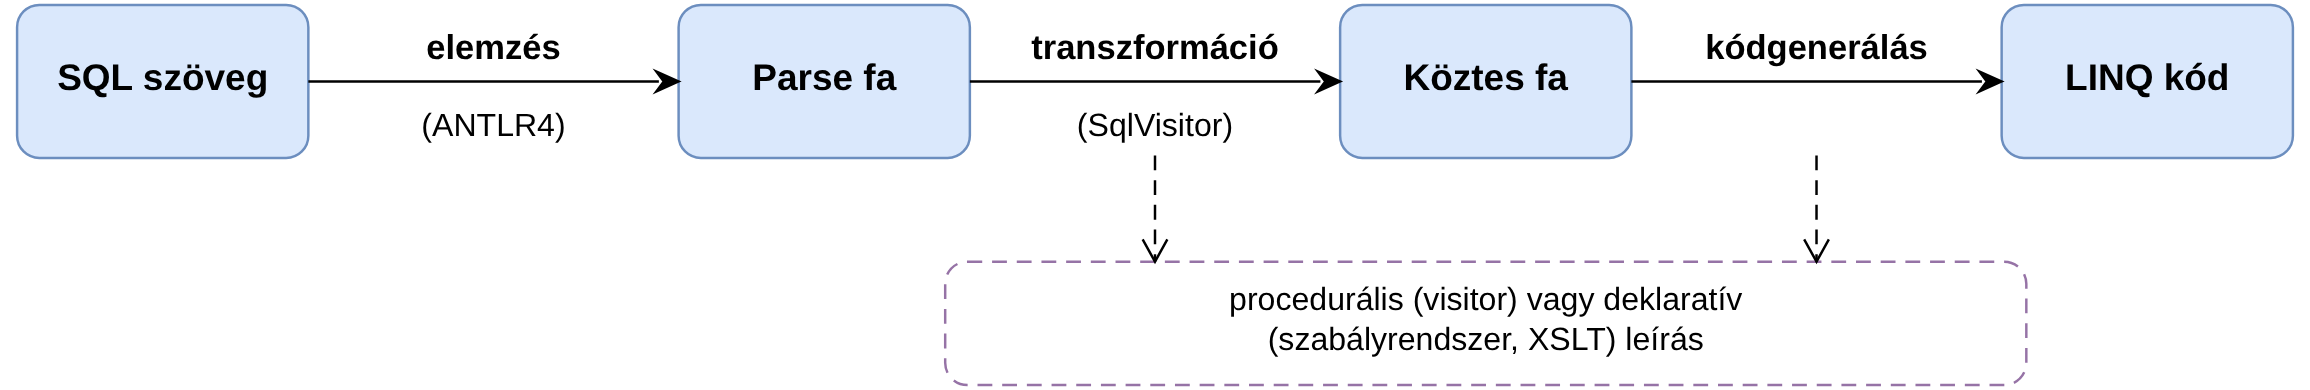
\includegraphics[width=\textwidth]{figures/forditasi_folyamat.png}
	\caption{Az SQL lekérdezések fordításának lépései}
	\label{fig:forditasi_folyamat}
\end{figure}

A transzformáció és a kódgenerálás egyaránt egy fa átalakítását jelenti, és mindkettő kétféleképpen írható le. Procedurális leírás esetén egy program járja be a fát, és minden csomóponttípushoz egy meghatározott lépéssorozatot hajt végre. Ennek tipikus megvalósítása a visitor tervezési minta \cite{gamma1994design}. Deklaratív leírás esetén az átalakítást szabályok halmaza adja meg. A szabályok azt írják le, hogy egy adott mintára illeszkedő csomópontból mi keletkezzen, az alkalmazásukról pedig egy általános feldolgozó gondoskodik. Ilyen például egy XSLT stíluslap vagy egy JSON, illetve YAML formátumú szabályrendszer. A procedurális leírás a környezetfüggő döntéseket közvetlenül kezeli, és a hibák nagy részét már a fordítóprogram jelzi. A deklaratív leírás ezzel szemben tömörebb, és a fordító újrafordítása nélkül is módosítható.

A dolgozat elsősorban a procedurális megközelítést mutatja be. A fordító megvalósítását, vagyis a grammatikát, a köztes fát és a visitor alapú transzformációt \aref{chap:megvalositas}. fejezet, a fordító helyességének ellenőrzését \aref{chap:teszteles}. fejezet ismerteti. \Aref{chap:llm}. fejezet a determinisztikus fordítót olyan nagy nyelvi modellekkel veti össze, amelyek a fordítást statisztikai alapon végzik. A deklaratív leírás lehetőségeit a kódgenerálás példáján \aref{chap:deklarativ}. fejezet vizsgálja, végül \aref{chap:altalanositas}. fejezet azt mutatja be, hogyan általánosítható a fordító más célnyelvek felé.

\Chapter{Szakirodalmi áttekintés}

A fordító több egymástól eltérő, de szorosan összefüggő kutatási területre támaszkodik: a for\-dí\-tó\-prog\-ram-elméletre és az ehhez kapcsolódó eszközökre, az objektum-relációs leképezés problémakörére, a LINQ és az Entity Framework Core belső működésére, valamint a transpilerek ipari alkalmazásaira.

\Section{Fordítóprogram-eszközök és az ANTLR}

A fordító megvalósításának alapját Terence Parr \textit{The Definitive ANTLR 4 Reference} \cite{parr2013antlr4} című munkája adja. Ez az átfogó referenciamű tárgyalja az ANTLR~4 parser generátor működését, a kontextusfüggetlen grammatikák írásának módszertanát, a lexer és parser automatikus előállítását, valamint a parse fa bejárásának két fő mintáját, a listener- és a visitor-alapú megközelítést. Az ANTLR~4 egyik legfontosabb újítása a korábbi verziókhoz képest az Adaptive~LL(*) (ALL*) algoritmus, amely a hagyományos LL(k) elemzőknél rugalmasabban kezeli a grammatikai kétértelműségeket és nem igényel bal-rekurzió eltávolítást. A projekt szempontjából különösen releváns a könyv visitor mintával foglalkozó fejezete, mivel a projekt látogató (visitor) alapú megközelítést használ. A látogató lehetővé teszi, hogy a parse fa bejárásakor minden csomóponttípushoz külön feldolgozási logikát rendeljünk, és a visszatérési értéket felfelé propagáljuk a fában. Ezt a mechanizmust alkalmazza a fordító \texttt{SqlVisitor} osztálya is.

Parr korábbi, \textit{Language Implementation Patterns} \cite{parr2009lip} munkája tágabb elméleti kontextusba helyezi az ANTLR-t és általában a nyelvfeldolgozás tervezési mintáit. A könyv külön mintaként tárgyalja a külső fa-látogatót (external tree visitor), amelynek lényege, hogy az AST csomópontjain végzett műveletek logikája elkülönül magától a fastruktúrától. Ez a szétválasztás lehetővé teszi, hogy ugyanazon szintaxisfát különböző célokra járjuk be anélkül, hogy a csomópontok definícióját módosítani kellene. A projekt is ezt az elvet követ. Az ANTLR által generált parse fán a \texttt{SqlVisitor} halad végig, és egy saját, a LINQ kódgeneráláshoz optimalizált absztrakt szintaxisfát (\texttt{LinqNode} hierarchiát) épít fel belőle. Ebből a fából aztán egy külön kódgenerátor, a \texttt{CSharpCodeGenerator} állítja elő a végleges C\# forráskódot, amely szintén látogatóként járja be a fát.

Ortin és társai \cite{ortin2022antlr} empirikus összehasonlítást végeztek az ANTLR és a hagyományos Lex/Yacc eszközpáros között. Eredményeik szerint az ANTLR szignifikánsan alacsonyabb fejlesztési időt és hibaarányt eredményez, különösen összetett, több alternatívát tartalmazó grammatikák esetén. Ez megerősíti az ANTLR választásának indokoltságát a projektben, ahol a teljes SQL \texttt{SELECT} szintaxis lefedése volt a cél.

\Section{Objektum-relációs impedancia-eltérés}

Az objektum-relációs impedancia-eltérés (Object-Relational Impedance Mismatch, ORIM) problémáját a szakirodalom régóta ismeri. Neward ezt a szembenállást találóan a számítástechnika Vietnámjaként jellemezte \cite{neward2006vietnam}, arra utalva, hogy az összekapcsolás látszólag egyszerű feladatnak tűnik, ám a megvalósítás során egyre mélyebb és nehezebben feloldható ellentmondások bukkannak fel. Ireland és társai \cite{ireland2009orim} strukturált keretrendszert dolgoztak ki az eltérések osztályozására, és négy fő kategóriát azonosítottak: adatmodell-eltérés (az objektumgráf és a relációs táblaszerkezet között), sémabeli eltérés (az öröklés és polimorfizmus vs.\ egyforma sorok), adatmanipulációs eltérés (az OOP metódushívásai vs.\ a halmazorientált SQL), valamint tranzakciós eltérés (az objektum életciklusa vs.\ a tranzakció határai). A fordító tervezésekor mindegyik kategória konkrét megvalósítási kihívásként jelentkezett. Például az SQL \texttt{NULL} kezelése alapvetően eltér a C\# nullable típusaitól, az SQL aggregátumok csoportosított adathalmazon értelmezettek, míg a LINQ aggregátumok az \texttt{IEnumerable} interfészen dolgoznak.

Papaioannou és Katsanos \cite{papaioannou2020orim} 2020-as empirikus vizsgálata az ORIM hatásait mérte ORM keretrendszerek teljesítményére. Eredményeik rávilágítanak arra, hogy az ORM által generált SQL lekérdezések egyes esetekben lényegesen kevésbé hatékonyak a kézzel írott megfelelőiknél, különösen összetett JOIN műveleteket és aggregációkat tartalmazó lekérdezéseknél. Ez a megfigyelés relevanciával bír a projekt egyik tervezési döntésénél, mivel a transpiler által generált LINQ kódnak nemcsak szintaktikailag kell helyesnek lennie, hanem az Entity Framework Core query provider számára szerver oldalon lefordíthatónak is, elkerülve a teljesítményt rontó kliensoldali kiértékelést.

\Section{LINQ és az Entity Framework Core}

A LINQ elméleti és gyakorlati hátterét Jon Skeet \textit{C\# in Depth} \cite{skeet2019csharp} munkája tárgyalja részletesen. A könyv különös figyelmet szentel a lusta kiértékelés (deferred execution) mechanizmusának, a kifejezésfa (expression tree) és az \texttt{IQueryable<T>} interfész kapcsolatának. Amíg a lekérdezés \texttt{IQueryable<T>} formában él, az EF Core képes azt kifejezésfaként elemezni és SQL-re fordítani. Amint azonban \texttt{IEnumerable<T>}-vé válik (pl.\ egy közbülső \texttt{ToList()} hívás következtében), az EF Core elveszti a SQL-generálás lehetőségét, és a kiértékelés C\# szinten, a memóriában folytatódik. A könyv továbbá hangsúlyozza, hogy a LINQ metódusszintaxisa (method syntax) és lekérdezési szintaxisa (query syntax) szemantikailag ekvivalens, azonban az előbbi programozottan könnyebben előállítható.

Freeman és Rattz \cite{freeman2010prolinq} könyve a LINQ teljes spektrumát lefedi. A projekt szempontjából különösen értékes a JOIN operátorok részletes tárgyalása. A \texttt{GroupJoin +} \\ \texttt{ SelectMany(DefaultIfEmpty)} kombináció mint a \texttt{LEFT OUTER JOIN} LINQ-beli megfelelője, az equi-join (.Join()) és a nem egyenlőség alapú (SelectMany + Where) JOIN-ok különbségei, valamint a több táblát érintő join-láncok felépítése. Ezek az ismeretek közvetlenül hasznosultak a fordító JOIN-kezelési logikájának tervezésekor.

A Microsoft hivatalos EF Core dokumentációja \cite{mslearn2023efcore} részletezi, hogy az EF Core provider egyes LINQ operátorokat (mint például a \texttt{GroupJoin}) nem minden adatbázis-provider esetén képes szerver oldalon SQL-re fordítani. Ez a korlát a projekt tesztelési infrastruktúrájában is konkrét kihívásként jelentkezett, mivel az SQLite provider nem fordítja szerver oldalra a \texttt{GroupJoin} alapú LEFT/RIGHT JOIN mintákat, ami azt jelenti, hogy a lánc kliensoldali LINQ-to-Objects módban fut le, ahol a \texttt{DefaultIfEmpty()} ténylegesen \texttt{null} objektumot szúr be, és az azt követő tulajdonság-hozzáférések \texttt{NullReferenceException}-t dobhatnak. Az outer join szemantikai tesztelésére ezért egy dedikált, null-mentes seed adatokkal dolgozó adatbázis-sémán történik.

\Section{A LINQ alkalmazása relációs adatbázisokon túl}

A LINQ tervezésének kiindulópontját Meijer, Beckman és Bierman \cite{meijer2006linq} munkája mutatja be. A szerzők célja egy olyan egységes lekérdezési modell kialakítása volt, amely az objektumgyűjtemények, a relációs adatok és az XML dokumentumok között nem tesz különbséget a programozó számára. Ezt a szabványos lekérdezőoperátorok és a cserélhető provider modell együttese teszi lehetővé. Ugyanaz a \texttt{Where}, \texttt{Select} vagy \texttt{OrderBy} hívás a memóriában tárolt gyűjteményen közvetlenül fut le, egy \texttt{IQueryable<T>} forrás esetén viszont kifejezésfaként jut el a providerhez, amely azt a saját célnyelvére fordítja. Ennek következtében a LINQ nem kötődik a relációs adatbázisokhoz, és több, egymástól lényegesen eltérő adatmodell lekérdezésére is alkalmazzák.

Az XML dokumentumok lekérdezésének hagyományos eszközei az XPath és az XQuery. A Microsoft dokumentációja \cite{mslearn2024xpathlinq} részletesen összeveti az XPath-t a LINQ to XML-lel, és a különbségek nagyrészt megegyeznek \aref{tab:adatbazis-eleres}. táblázatban bemutatott, SQL stringek és LINQ közötti különbségekkel. Az XPath kifejezés egy string, amelyet a fordítóprogram nem elemez, így a hibák csak futásidőben derülnek ki, az eredmény pedig gyakran típus nélküli objektum, amelyet a fejlesztőnek kell a megfelelő típusra alakítania. A LINQ to XML lekérdezéseit ezzel szemben a C\# fordító ellenőrzi, a vetítések típusosak, és a lekérdezés eredménye nem csak a fa csomópontjaiból állhat, hanem tetszőleges új objektumból vagy XML szerkezetből is. A dokumentáció az XPath tengelyek többségéhez közvetlen LINQ to XML megfelelőt ad meg (a \texttt{child} tengelynek például az \texttt{Elements()}, a \texttt{descendant} tengelynek a \texttt{Descendants()} metódus felel meg), a \texttt{following} és \texttt{preceding} tengelyeknek azonban nincs közvetlen megfelelőjük. Ez a helyzet a jelen munkában vizsgált leképezéshez hasonló, ahol szintén a forrásnyelv egy jól körülhatárolható részhalmaza fordítható közvetlenül.

A dokumentumorientált adatbázisok területén a MongoDB 2024 májusában tette általánosan elérhetővé saját Entity Framework Core providerét, amely az EF Core 8 és a .NET 8 platformot támogatja \cite{mongodb2024efcore}. A provider a code-first megközelítést, az alapvető CRUD műveleteket, a beágyazott dokumentumokat és a változáskövetést kezeli, a lekérdezések oldalán pedig a \texttt{Where}, \texttt{OrderBy} és \texttt{ThenBy} operátorokat, valamint az aggregátumokat fordítja le. A provider dokumentációja ugyanakkor számos korlátot is felsorol \cite{mongodb2024limitations}. Nem támogatottak a migrációk és az idegen kulcsok, és a jelenlegi változat nem kezeli az eredményt átalakító \texttt{Select} vetítéseket sem, beleértve a névtelen típusokba történő vetítést. A projekt szempontjából ez a korlát különösen tanulságos, mivel a fordító a többoszlopos \texttt{SELECT} utasításokat éppen névtelen objektumot előállító \texttt{Select} hívásra képezi le. A generált kód tehát szintaktikailag helyes maradna, ezen a provideren mégsem lenne futtatható. Ez jól szemlélteti, hogy egy LINQ kifejezés futtathatósága nem csak a nyelvtől, hanem a mögötte álló providertől is függ.

A HTML dokumentumok feldolgozására az AngleSharp .NET könyvtár kínál LINQ alapú megoldást \cite{anglesharp}. A könyvtár a W3C szabványnak megfelelő DOM-ot valósít meg, amelyben a csomópontok a böngészőkből ismert \texttt{QuerySelector} és \texttt{QuerySelectorAll} metódusokkal, CSS szelektorok segítségével kereshetők, a DOM összes gyűjteménye pedig LINQ lekérdezésekkel tovább feldolgozható. A szelektorral kiválasztott elemekre így közvetlenül láncolható egy \texttt{Where} szűrés vagy egy \texttt{Select} vetítés. Az AngleSharp esetében a lekérdezés a LINQ to XML-hez hasonlóan a memóriában, LINQ to Objects módban fut le, és nincs olyan provider, amely a kifejezést más nyelvre fordítaná.

A bemutatott példák alapján a LINQ alkalmazásai két csoportba sorolhatók. Az első csoportban (LINQ to XML, AngleSharp) a lekérdezés a memóriában tárolt adatszerkezeten közvetlenül hajtódik végre, és a LINQ egy típusbiztos, a stringalapú lekérdezőnyelveket kiváltó API szerepét tölti be. A második csoportban (EF Core, MongoDB provider) a lekérdezés kifejezésfaként jut el a providerhez, amely azt egy másik lekérdezőnyelvre fordítja, így a provider képességei határozzák meg, hogy mely LINQ konstrukciók használhatók. A jelen munkában bemutatott fordító a második csoporthoz kapcsolódik, a vizsgált területek pedig további továbbfejlesztési irányokat jelölnek ki, például egy MongoDB providerhez igazodó vagy XPath kifejezéseket feldolgozó fordító formájában.

\Section{Roslyn és kódgenerálás}

A jelen projekt tesztelési infrastruktúrájában a Microsoft Roslyn fordítóplatform is szerepet kapott. Vasani \cite{vasani2017roslyn} és Harrison \cite{harrison2017codegen} munkái részletesen tárgyalják a Roslyn \textit{Compiler as a Service} megközelítést, amelynek keretében a C\# fordítófolyamat programozottan érhető el, lehetővé téve szintaktikai fák elemzését, szemantikai modellezést, kódgenerálást, valamint dinamikus kódfordítást és futtatást memóriában. A \texttt{FuzzTests} osztály a Roslyn \\ \texttt{SyntaxFactory.ParseExpression()} metódusát alkalmazza a generált LINQ kifejezések szintaktikai érvényességének ellenőrzésére. Ez lehetővé teszi, hogy véletlenszerűen generált SQL lekérdezések LINQ-ra fordított kimenete szintaxishibák szempontjából anélkül legyen vizsgálható, hogy az érintett táblák valóban léteznének az adatbázisban.

\Section{Transpilerek az iparban}

Az nMorph keretrendszer \cite{nmorph2023} egy transpiler-alapú megközelítést mutat be több programozási nyelvet érintő szoftverfejlesztési problémák megoldására. A keretrendszer rávilágít arra, hogy a transpiler-technológia nemcsak kód-migrációra alkalmazható, hanem általánosabb, többnyelvű szoftverfejlesztési munkafolyamatok automatizálásának eszközeként is.

Borne \cite{borne2021transpiler} esettanulmánya egy valódi ipari transpiler megvalósítását mutatja be, amely egy Oracle PL/SQL kódbázist fordít PostgreSQL-re. A cikk részletezi a megközelítés architektúráját, és hangsúlyozza, hogy az automatizált kódfordítás soha nem lehet teljes körű, mivel bizonyos konstrukciók, amelyek az egyik rendszerben természetesek, a másikban nem fejezhetők ki közvetlenül. Ez a megfigyelés összhangban van a projekt során szerzett tapasztalatokkal, mivel a SQL nyelv egyes elemei, például a \texttt{FULL OUTER JOIN}, a közös táblakifejezések (CTE) és az ablakfüggvények (\texttt{ROW\_NUMBER}, \texttt{RANK}) nem rendelkeznek LINQ-ban olyan közvetlen megfelelővel, amely az Entity Framework Core által szerveroldali SQL-lekérdezéssé fordítható. Emiatt ezeknek a konstrukcióknak a támogatása a transpiler jelenlegi hatókörén kívül esik.

Az SQL lekérdezések LINQ-ra fordítására kereskedelmi eszköz is létezik. A Linqer \cite{linqer} egy 2011-es ismertetés \cite{selmani2011linqer} szerint SQL lekérdezésekből LINQ to SQL vagy LINQ to Entities modellhez illeszkedő, C\# vagy Visual Basic nyelvű kódot állít elő, lekérdezési szintaxisban. A jelen fordító ettől több szempontból különbözik. Metódusszintaxist állít elő, amely az EF Core 8 szerveroldali fordításához igazodik, a kimenet helyességét pedig string-szintű és szemantikai ekvivalencia tesztek igazolják. A forráskód nyilvánosan elérhető, a fordító könyvtárként saját projektbe is beépíthető.

\Chapter{Megvalósítás}
\label{chap:megvalositas}

A fejezet a fordító tervezését és megvalósítását mutatja be.

\Section{A tervezési döntések háttere}

A fordító tervezésekor az első és legfontosabb kérdés az volt, hogy milyen szintű absztrakcióban érdemes gondolkodni. Az egyik szélsőséges megközelítés a közvetlen szöveges transzformáció lett volna, ahol a bemeneti SQL string reguláris kifejezések és szövegcserék útján alakul át LINQ kóddá. Ez a megközelítés egyszerűnek tűnik kis méretű, szabályos bemeneteken, de az SQL nyelv kontextusfüggő természete miatt gyorsan kezelhetetlenné válik. Egy feltétel például másképpen viselkedik \texttt{WHERE} záradékban, \texttt{HAVING} záradékban, allekérdezés belsejében vagy \texttt{CASE WHEN} kifejezésben, és ezeket a különbségeket reguláris kifejezéssel nem lehet megbízhatóan felismerni.

A másik véglet egy teljes fordítóprogram-lánc lett volna saját lexerrel, parserrel és szemantikai elemzővel. Ez ugyan a lehető legrugalmasabb megoldást adta volna, de az implementáció terhe aránytalanul nagynak tűnt a projekt céljaihoz képest, és a karbantarthatóságot is megnehezítette volna.

A két véglet között szóbajöhető megközelítések közül egy háromrétegű architektúra bizonyult a legjobb megoldásnak.
\begin{itemize}
	\item Az első réteg egy ANTLR4-gyel generált parser, amely az SQL szöveget parse fává alakítja.
	\item A második réteg egy saját absztrakt szintaxisfa, amely a LINQ-specifikus struktúrákat reprezentálja.
	\item A harmadik réteg a tényleges kódgenerátor, amely ebből az absztrakt reprezentációból állítja elő a végleges C\# forráskódot.
\end{itemize}
Ez a szétválasztás több előnnyel is jár. A grammatika és a kódgenerálás egymástól függetlenül fejleszthető és tesztelhető. Új SQL konstrukciók bevezetésekor elegendő egy új grammar szabályt, egy új AST-csomópontot és egy új visitor metódust hozzáadni, a rendszer többi része változatlan marad.

A fordítási folyamat lépéseit \aref{fig:pipeline_forditas}. ábra szemlélteti.

\begin{figure}[H]
	\centering
	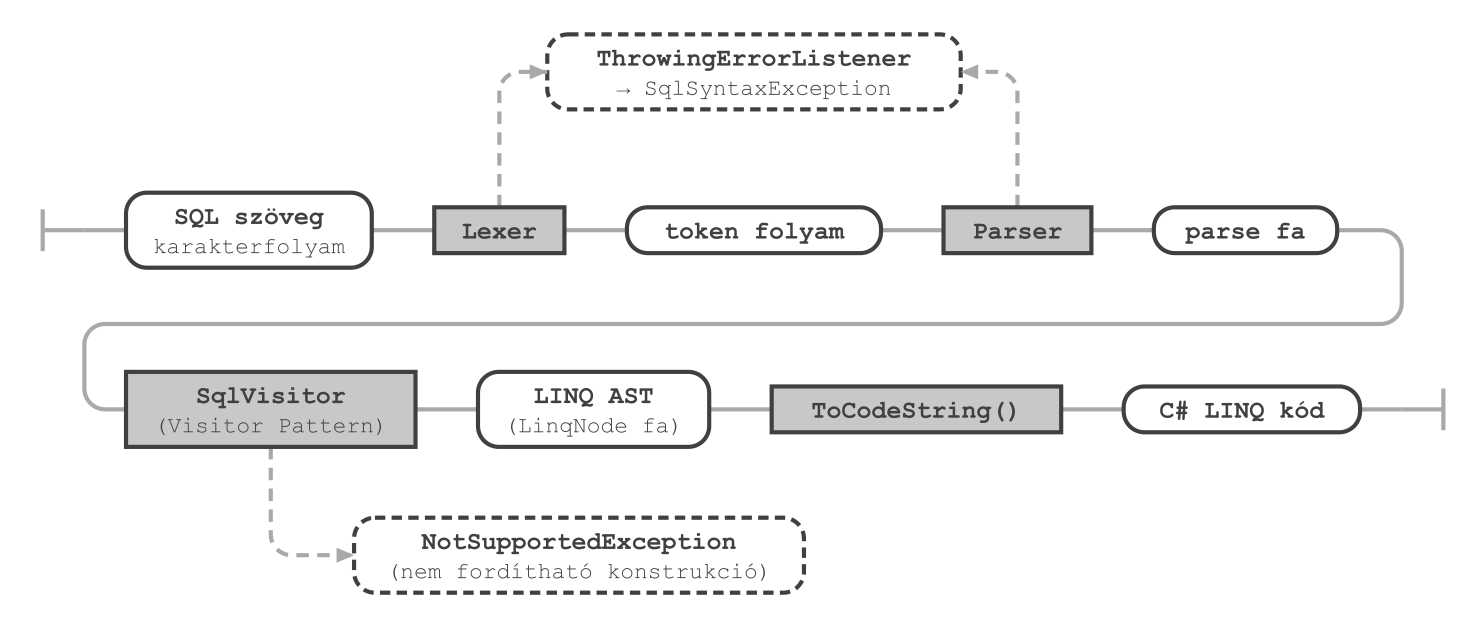
\includegraphics[width=\textwidth]{figures/pipeline_forditas.png}
	\caption{A fordítási pipeline lépései}
	\label{fig:pipeline_forditas}
\end{figure}

\Section{A grammatika és a parser}

A parser előállításához az ANTLR4 parser generátor mellett döntöttem. Az ANTLR4 kontextusfüggetlen grammatikából automatikusan generál lexert és parsert, amelyek a bemeneti szöveget parse fává alakítják. A kontextusfüggetlen grammatikák és az elemzési fák fogalmát a formális nyelvek elmélete írja le \cite{bach2002formalis}. A generált kód C\# nyelvű, így közvetlenül integrálható a .NET alapú projektbe.

Az SQL grammatika megírása során fontos szempont volt, hogy a nyelvtan csak azt fedje le, amit a fordító valóban képes kezelni. Egy teljes SQL:1999-es grammatika hatalmas, és sok olyan konstrukciót tartalmaz amelynek LINQ-ban nincs közvetlen megfelelője. A projekt grammatikája ezért szándékosan az SQL nyelv egy szűkebb, de teljes egészében támogatott részhalmazát fedi le, amelynek minden szabályához rendelkezésre áll a megfelelő LINQ-kódgenerálási logika.

A szűkítés két szinten történt. Az utasítások szintjén a grammatika legfelső \texttt{query} szabálya csak a \texttt{SELECT}, \texttt{INSERT}, \texttt{UPDATE} és \texttt{DELETE} utasításokat ismeri. Az adatdefiníciós (DDL), a jogosultságkezelő és a tranzakciókezelő utasítások így már a szintaktikai elemzés során \texttt{SqlSyntaxException} kivételt váltanak ki. Az utasításokon belül egy konstrukció csak akkor került be a grammatikába, ha a fordító determinisztikus, az EF Core által szerveroldalon is lefordítható LINQ megfelelőt tud hozzá előállítani. Ennek megfelelően kimaradt többek között a \texttt{FULL OUTER JOIN}, a közös táblakifejezések (\texttt{WITH ... AS}), az ablakfüggvények és a \texttt{NULLS FIRST} / \texttt{NULLS LAST} rendezési módosítók. A \texttt{LEFT} és \texttt{RIGHT} szövegfüggvények sem támogatottak, mivel ezek a szavak a grammatikában a join típusok kulcsszavai. A grammatika bővítése iteratívan történt, egy új szabály a hozzá tartozó kódgenerálási logikával és tesztesetekkel együtt került be.

Vannak olyan konstrukciók is, amelyeket a grammatika szintaktikailag elfogad, de a visitor csak bizonyos alakjukban tud lefordítani. Ilyen például a nem egyenlőségen alapuló \texttt{LEFT JOIN} feltétel, a szöveges operandusokra alkalmazott \texttt{BETWEEN}, vagy a \texttt{COUNT}-on kívüli \\ \texttt{DISTINCT} aggregátum. Ezekben az esetekben a visitor \texttt{NotSupportedException} kivétellel, a konstrukciót megnevező hibaüzenettel jelzi, hogy a bemenet nem fordítható. A szűkítés tehát kétlépcsős. A szintaktikai szint kiszűri a fordító hatókörén kívül eső utasításokat, a szemantikai szint pedig az elvileg érvényes, de megbízhatóan nem fordítható alakokat.

A szűkítés mértékét a grammatika mérete is jól mutatja. A projekt grammatikája 37 parser szabályból és 69 lexer szabályból áll, utóbbiak közül 49 kulcsszó, és a teljes nyelvtan 156 nem üres sort tesz ki. Ezzel szemben az SQL:1999 szabvány teljes nyelvtana több száz szabályt tartalmaz.

A lexer a bemeneti karakterfolyamból tokeneket állít elő. A kulcsszavak esetében figyelmen kívül hagyja a kis- és nagybetű különbséget, így a \texttt{SELECT}, \texttt{select} és \texttt{Select} alakok egyenértékűek. Az azonosítók felismerése után a fordító egy \texttt{ToPascalCase} konverziót végez, amely az SQL konvencióinak megfelelő \texttt{snake\_case} vagy csupa nagybetűs neveket C\#-ban szokásos PascalCase formára hozza. Ez azt jelenti, hogy a \texttt{user\_name} oszlopnévből automatikusan \texttt{UserName}, a \texttt{USERS} táblanévből pedig \texttt{Users} lesz.

A nyelvtan felépítése a legáltalánosabb szabályoktól halad a specifikusak felé. A legfelső szintű \texttt{query} szabály a négy támogatott utasítástípus egyikét várja \\ (\texttt{selectQuery}, \texttt{deleteStmt}, \texttt{insertStmt} vagy \texttt{updateStmt}), amelyet tetszőleges számú pontosvessző követhet. A \texttt{selectQuery} lehetőséget ad halmazműveletek láncolására (\texttt{UNION}, \texttt{INTERSECT}, \texttt{EXCEPT}), míg maga a \texttt{selectStmt} bontja ki az egyes lekérdezések szerkezetét. A \texttt{condition} szabály rekurzív, ami lehetővé teszi az \texttt{AND}, \texttt{OR} és \texttt{NOT} operátorok tetszőleges mélységű egymásba ágyazását. Az \texttt{expr} szabály szintén rekurzív, kezelve az aritmetikai kifejezéseket és a allekérdezéseket. Az ANTLR4 Adaptive~LL(*) algoritmusának köszönhetően ezek a rekurzív szabályok kezelhetők anélkül, hogy kézzel kellene foglalkozni a kétértelműségekkel.

A grammatika egyik legösszetettebb szabályának, a \texttt{condition}-nek a railroad diagramját \aref{fig:rr_condition}. ábra mutatja. A további főbb szabályok diagramjai \aref{sec:rr_melleklet}. mellékletben találhatók.

\begin{figure}[H]
	\centering
	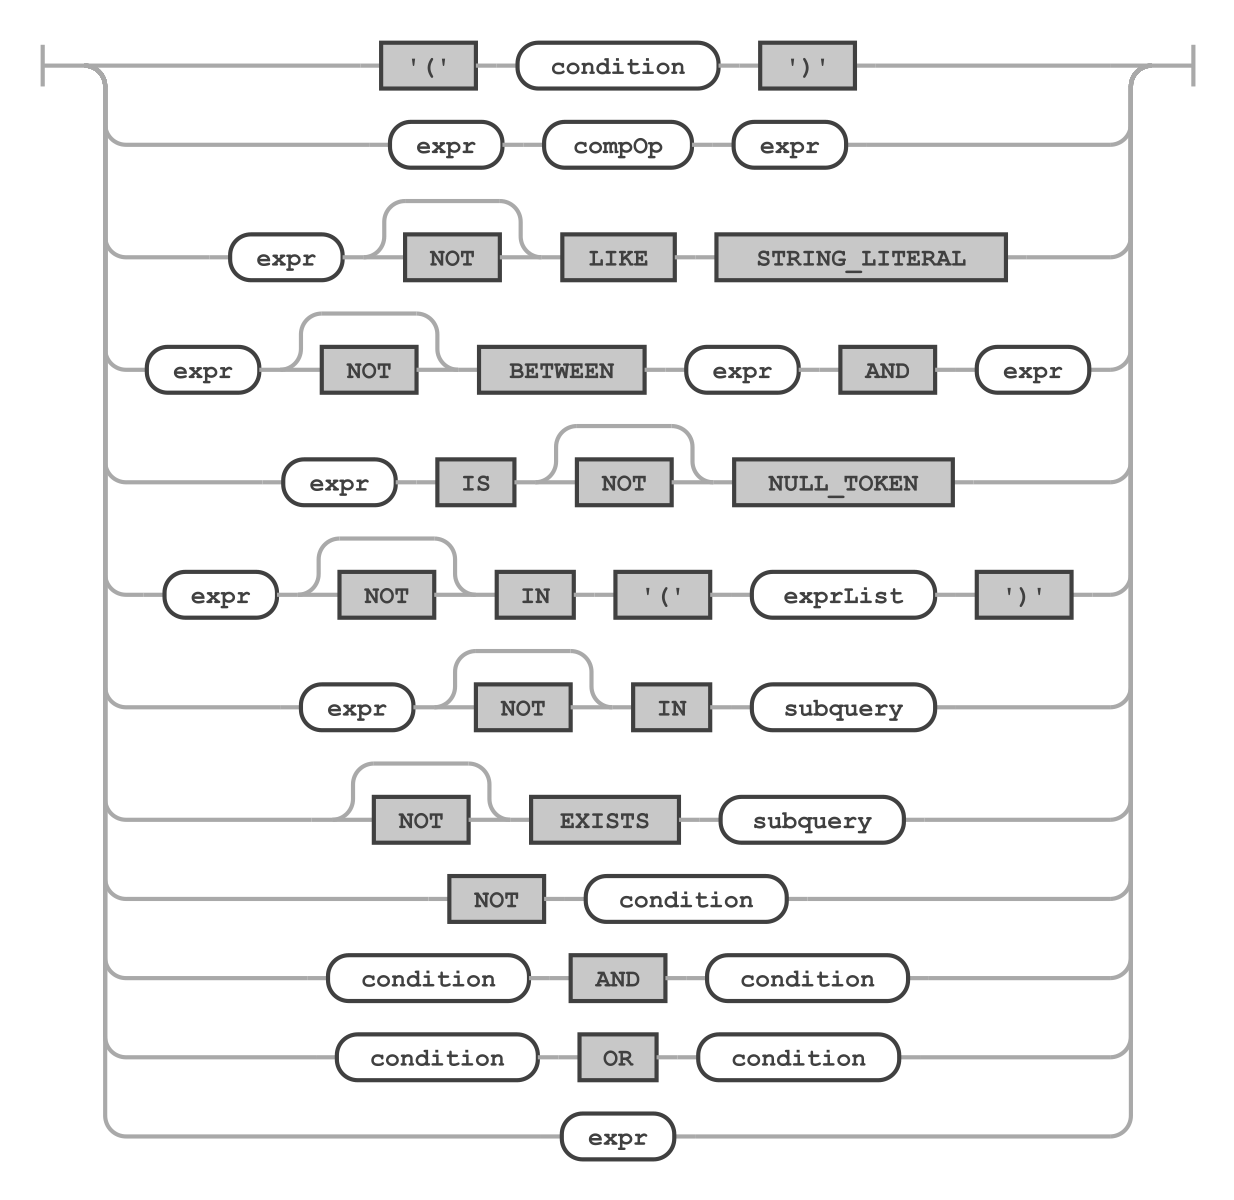
\includegraphics[width=\textwidth]{figures/condition.png}
	\caption{A \texttt{condition} grammatikai szabály railroad diagramja}
	\label{fig:rr_condition}
\end{figure}

A többargumentumú függvényhívások kezelésére a grammatika egy variadikus szabályt alkalmaz. Az első változatban a két-, három- és négyargumentumú esetekre külön-külön szabályok léteztek, amit egy általánosabb \texttt{funcCallExpr} szabály váltott fel, amely \\ \texttt{expr (COMMA expr)+} alakban írható le. Ez a változtatás egyszerűsítette a nyelvtant és lehetővé tette, hogy az argumentumszám-érvényesítés a visitor rétegbe kerüljön, ahol értelmes hibaüzenettel jelezhető, ha egy függvényt helytelen számú paraméterrel hívnak meg.

\Section{Az absztrakt szintaxisfa}

Az ANTLR4 által generált parse fa az SQL szintaxis közvetlen tükörképe, mivel minden grammatikai szabályhoz egy-egy csomópont tartozik. Ez a reprezentáció a kódgenerálás szempontjából túlságosan alacsony szintű, mert olyan részleteket tartalmaz amelyek a LINQ kód előállításához irrelevánsak, például a zárójeleket, a vesszőket és az SQL kulcsszavakat. Emiatt a fordító egy saját absztrakt szintaxisfát épít fel, amelynek csomópontjai már a LINQ struktúráknak megfelelő fogalmakat reprezentálnak.

A csomóponthierarchia alapja az absztrakt \texttt{LinqNode} osztály. Minden konkrét csomóponttípus ebből öröklődik, és egyetlen kötelező metódusa, az \texttt{Accept()}, a fát bejáró látogatónak adja át a vezérlést. A csomópontok nem tartalmaznak célnyelvi kódot, csak a lekérdezés szerkezetét írják le.

A \texttt{LinqQueryNode} tárolja a forrástábla nevét és a metódushívások rendezett listáját, ez képviseli az egész lekérdezést. A \texttt{LinqMethodCallNode} egyetlen LINQ metódushívást ír le, névvel és argumentumlistával. \\A \texttt{LinqLambdaNode} egy lambda kifejezést tartalmaz paraméternévvel és törzs\-zsel, és ez jelenik meg a \texttt{Where}, \texttt{Select}, \texttt{OrderBy} és hasonló metódusok belső kifejezéseként.

A \texttt{LinqAnonymousObjectNode} egy névtelen C\# objektumot reprezentál, amelyet a többoszlopos \texttt{SELECT} vetítések állítanak elő.

A \texttt{LinqJoinNode} a \texttt{JOIN} konstrukciót modellezi, tárolja a join típusát, a belső tábla nevét, valamint a bal és jobb oldali kulcskifejezést.

A kifejezések szintjén a \texttt{LinqConstantNode} literális értékeket tárol, a \\ \texttt{LinqIdentifierNode} azonosítókat és oszlophivatkozásokat, \\a \texttt{LinqBinaryExpressionNode} bináris kifejezéseket (aritmetika, összehasonlítás), a \\ \texttt{LinqCaseNode} pedig a \texttt{CASE WHEN} szerkezetet modellezi, tárolja az opcionális operandust, a \texttt{WHEN} ágak listáját és az \texttt{ELSE} kifejezést.

A DML utasítások saját gyökércsomópontokat kaptak. A \texttt{LinqDeleteNode} a törlési utasítást reprezentálja a forrástábla nevével, az opcionális \texttt{WHERE} feltétellel és a lambda paraméternévvel. A \texttt{LinqInsertNode} a \texttt{VALUES} alapú beszúrást tárolja, soronként tartalmazza az oszlopnév-érték párokat. A \texttt{LinqInsertSelectNode} az \texttt{INSERT INTO ... SELECT} alakot kezeli, tárolja a céltáblát, az oszloplistát és a teljes SELECT lekérdezés AST-jét, amelyből kódgeneráláskor a projekciót újra kell írni. A \texttt{LinqUpdateNode} az \texttt{UPDATE} utasítást modellezi a \texttt{SET} értékadások listájával, amelynek minden eleme egy \\ \texttt{(ColumnName, LinqNode)} pár.

Ez az elrendezés teszi lehetővé, hogy a kódgenerálás egyszerűen a cso\-mó\-pont-fa bejárásával valósuljon meg. Egy lekérdezés generálásához elegendő a kódgenerátor \texttt{Generate()} metódusát a gyökér \texttt{LinqQueryNode} csomóponttal meghívni. A generátor minden csomóponttípushoz külön \texttt{Visit...} metódust tartalmaz, amely a gyermek csomópontok kódját rekurzívan előállítja, és az eredményeket összefűzi.

A LINQ kód egy lánc alakú metódushívás-sorozat, amelynek sorrendje kötött. A fordítónak ezt a sorrendet be kell tartania. Az AST-alapú megközelítés ezt természetesen kezeli, mivel a \texttt{LinqQueryNode} a metódusokat egy rendezett listában tárolja, és a visitor réteg gondoskodik arról, hogy ezek a helyes sorrendben kerüljenek bele.

Érdemes megfigyelni, hogy a két fa szerkezete lényegesen eltér egymástól. \Aref{fig:parse_fa_q1}. és \aref{fig:koztes_fa_q1}. ábra ugyanannak a \texttt{SELECT Name, Age FROM Users WHERE Age > 18 } \\ \texttt{ORDER BY Name ASC} lekérdezésnek a két fáját mutatja. A parse fa 39 csomópontból áll, ezek közül 15 levél. A levelek az egyes tokenek, vagyis a kulcsszavak, az azonosítók, a literálok és az írásjelek. Minden grammatikai szabály külön szintet ad a fához, ezért egy egyszerű oszlopnév is csak a \texttt{selectItem}, az \texttt{expr} és az \texttt{identifier} csomópont alatt jelenik meg.

\begin{figure}[H]
	\centering
	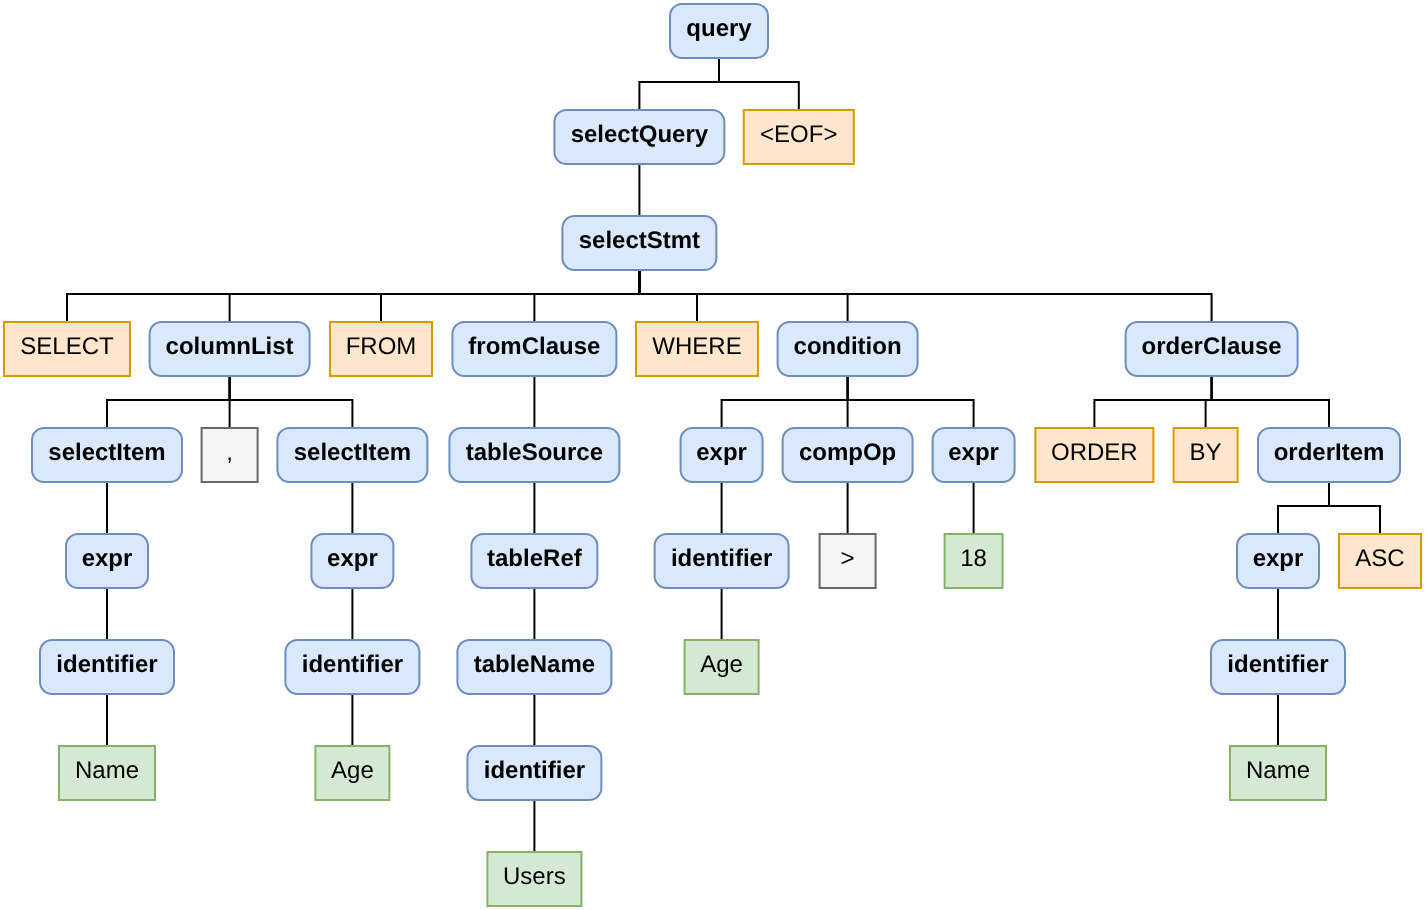
\includegraphics[width=\textwidth]{figures/parse_fa_q1.png}
	\caption{A \texttt{SELECT Name, Age FROM Users WHERE Age > 18 ORDER BY Name ASC} lekérdezés parse fája. Kék színnel a grammatikai szabályok, narancssárgával a kulcsszavak, zölddel az azonosítók és a literálok, szürkével az írásjelek és az operátorok láthatók.}
	\label{fig:parse_fa_q1}
\end{figure}

A köztes fában ugyanehhez a lekérdezéshez 19 csomópont tartozik. A kulcsszavak és az írásjelek eltűnnek, a gyökér \texttt{Query} csomópont gyermekei pedig a LINQ metódusláncot követik. A \texttt{SELECT} záradék a parse fában az első helyen áll, a köztes fában viszont a \texttt{Select} hívás a szűrés és a rendezés után következik, mert a metódusok abban a sorrendben szerepelnek, ahogyan a generált kódban. A metódusok argumentumai lambda csomópontok, ezek törzsében pedig kifejezéscsomópontok állnak, például tagelérés, bináris kifejezés és konstans. Ez a szétválasztás teszi egyszerűvé a kódgenerálást, mivel a fa bejárásakor már csak a LINQ szerkezetnek megfelelő csomópontokkal kell foglalkozni.

\begin{figure}[H]
	\centering
	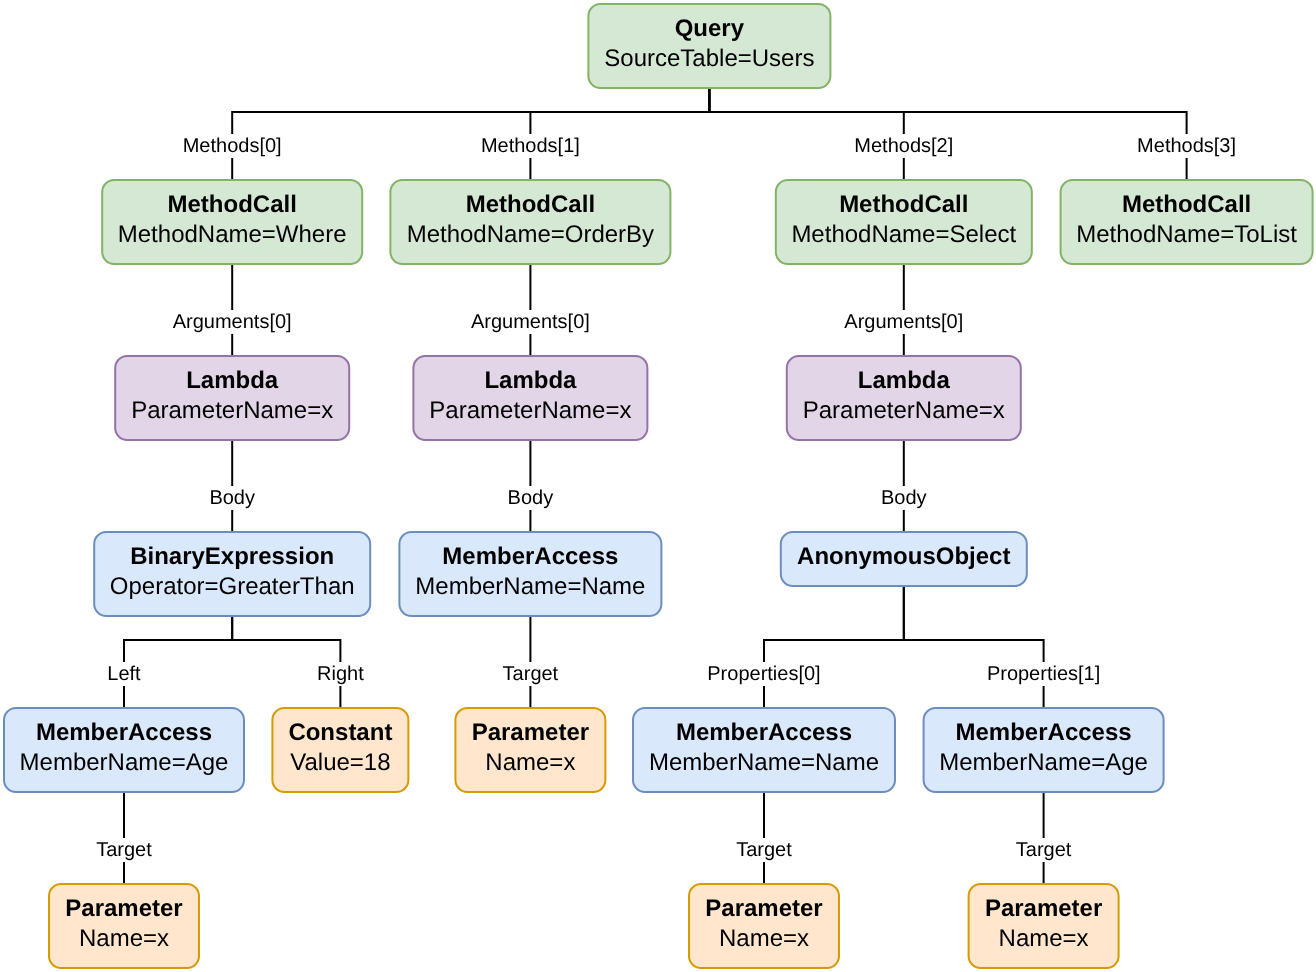
\includegraphics[width=\textwidth]{figures/koztes_fa_q1.png}
	\caption{Ugyanennek a lekérdezésnek a köztes fája. Zöld színnel a lekérdezés és a metódushívások, lilával a lambda kifejezések, kékkel a további kifejezéscsomópontok, narancssárgával a paraméterek és a konstansok láthatók. Az éleken a csomópont azon tulajdonságának neve áll, amely a gyermekre hivatkozik.}
	\label{fig:koztes_fa_q1}
\end{figure}

A különbség az összetettebb lekérdezéseknél is megmarad. \Aref{tab:fameret}. táblázat az LLM-mérés öt lekérdezésének fáit hasonlítja össze. A köztes fa minden esetben a parse fa csomópontjainak 39--49 százalékát tartalmazza, kevesebb szintből áll, és a legszélesebb szintje két-háromszor keskenyebb.

\begin{table}[H]
	\centering
	\renewcommand{\arraystretch}{1.4}
	\small
	\begin{tabular}{|l|c|c|c|c|}
		\hline
		\textbf{Lekérdezés} & \textbf{Csomópontok} & \textbf{Levelek} & \textbf{Mélység} & \textbf{Szélesség} \\
		\hline
		Q1 & 39 / 19 & 15 / 6 & 9 / 6 & 10 / 5 \\
		\hline
		Q2 & 62 / 25 & 30 / 9 & 9 / 6 & 16 / 7 \\
		\hline
		Q3 & 85 / 33 & 38 / 11 & 9 / 7 & 19 / 7 \\
		\hline
		Q4 & 103 / 40 & 46 / 14 & 13 / 11 & 22 / 7 \\
		\hline
		Q5 & 147 / 62 & 68 / 21 & 10 / 10 & 36 / 12 \\
		\hline
	\end{tabular}
	\caption{A parse fa és a köztes fa mérete az öt mért lekérdezésnél. Minden cellában az első érték a parse fára, a második a köztes fára vonatkozik. A mélység a szintek száma, a szélesség a legtöbb csomópontot tartalmazó szint mérete.}
	\label{tab:fameret}
\end{table}

\Section{A SELECT fordítása}

Az alfejezetben a \texttt{SELECT} utasítások fordítási módja kerül részletezésre.

\SubSection{A visitor és a scope kezelés}

A parse fa bejárására az ANTLR4 visitor mintáját alkalmazom. Az ANTLR4 a grammatikából automatikusan generálja az alap visitor interfészt, amelyet a \texttt{SqlVisitor} osztály implementál. Minden grammatikai szabályhoz egy \texttt{Visit...} metódus tartozik, amely a megfelelő \texttt{LinqNode} leszármazottat építi fel és adja vissza.

A visitor legösszetettebb része a scope kezelés, amelyre az SQL allekérdezések és korrelált hivatkozások miatt van szükség. Amikor egy belső \texttt{SELECT} lekérdezés hivatkozik a külső lekérdezés egy táblájára vagy aliasára, a fordítónak el kell döntenie, hogy az adott azonosítót melyik lambda paraméterrel kell prefixelni. Erre a célra az \texttt{\_outerScopes} nevű verem szolgál, amelybe minden \texttt{SELECT} feldolgozásának kezdetén bekerül az aktuális tábla-alias leképezés és az aktuális lambda paraméter neve. Amikor a belső lekérdezés egy azonosítót nem talál meg a saját scope-jában, végigmegy a veremben lévő elemeken és megkeresi a névhez tartozó (legközelebbi/legszűkebb) külső scope-ot, majd az ott tárolt lambda paramétert használja prefixként. (Névfeloldási hiba így tehát csak akkor keletkezik, hogy ha egyetlen scope-ban sem található meg a keresett név.) Egy korrelált \texttt{EXISTS} allekérdezés fordítását \aref{lst:korrelalt}. kódpélda mutatja be.

\begin{lstlisting}[caption={Korrelált allekérdezés scope kezelése}, label={lst:korrelalt}]
	// Korrelált EXISTS allekérdezés generálása
	// SQL: SELECT Name FROM Users u WHERE EXISTS 
	//        (SELECT 1 FROM Orders o WHERE o.Owner = u.Id)
	// Generált LINQ:
	db.Users.Where(x => (db.Orders.Where(o => o.Owner == x.Id)).Any())
	.Select(x => new { x.Name })
	.ToList()
\end{lstlisting}

A lambda paraméter nevének nyomon követése nem triviális. Az egyszerű, alias nélküli lekérdezésekben a lambda paraméter mindig \texttt{x}. Ha azonban a lekérdezésben explicit SQL alias szerepel, például \texttt{FROM Orders o}, a belső lambda paraméter neve az alias lesz, tehát \texttt{o}. Ez biztosítja, hogy a generált kód olvasható maradjon, és a korrelált hivatkozások egyértelműen azonosíthatóak legyenek a generált LINQ-ban.

A \texttt{GROUP BY} kontextus kezelése szintén különleges figyelmet igényel. A csoportosítás után a LINQ \texttt{Select} metódus lambda paraméterként a \texttt{g} csoportváltozót kapja, az oszlophivatkozások pedig \texttt{g.Key} vagy \\\texttt{g.First\-OrDefault().Oszlop} alakot öltenek. A visitor nyilvántartja, hogy éppen \\ \texttt{GROUP BY} kontextusban dolgozik-e, és ennek megfelelően módosítja a generált kifejezéseket. Egy belső allekérdezés látogatásakor a kontextus flag-ek mentésre kerülnek, és a belső lekérdezés feldolgozása után visszaállítódnak, hogy a külső lekérdezés kontextusa ne sérüljön.

A kód olvashatóságának és karbantarthatóságának javítása érdekében a fejlesztés során több ismétlődő minta kiszervezésre került újrafelhasználható segédmetódusokba. A \\ \texttt{BuildWhereMethod} metódus elvégzi a \texttt{\_inWhereClause} flag beállítását, a feltétel látogatását és a \texttt{LinqMethodCallNode} összerakását. Hasonlóan, a \texttt{BuildOrderByMethods} az \texttt{ORDER BY} záradék feldolgozását végzi, a \texttt{SetupTableScope} pedig a tábla-alias leképezés és a scope verem feltöltését. Ezek a segédmetódusok egységes belépési pontot biztosítanak, és lehetővé teszik, hogy a \texttt{DELETE} és az \texttt{UPDATE} utasítások is ugyanazokat a WHERE és ORDER BY generálási logikákat használják, amelyek a \texttt{SELECT} esetén megvalósításra kerültek.

\SubSection{Kódgenerálás}

A kódgenerálást a \texttt{CSharpCodeGenerator} osztály végzi, amely a visitor által felépített köztes fát rekurzívan járja be. A folyamat kiindulópontja mindig a gyökér \texttt{LinqQueryNode}, amelynek kódja a forrástábla nevével kezdődik (\texttt{db.Tabla}), majd ehhez sorban hozzáfűződik a \texttt{Methods} lista elemeiből generált kód.

A többoszlopos \texttt{SELECT} esetén a \texttt{LinqAnonymousObjectNode} csomópontból névtelen C\# objektum keletkezik. Ha az oszlop neve megegyezik a forrásoszlop nevével, a generátor egyszerű, közvetlen névhasználatot (\textit{shorthand}-et) alkalmaz (\texttt{x.Nev}), különben explicit hozzárendelést (\texttt{Alias = x.Nev}). A \texttt{SELECT *} speciális eset, ahol nem keletkezik \texttt{Select} metódushívás, csak a \texttt{ToList()} zárja a láncot.

Az allekérdezések generálása során fontos különbséget tenni a skaláris és a kollekcióalapú allekérdezések között. Az \texttt{IN (SELECT ...)} esetén a belső lekérdezés skaláris projekciót kap, és az összehasonlítás \texttt{Any()} metódussal történik, amely típusbiztos és nullable típusokat is helyesen kezel. Kivételt képez az az eset, amikor a belső lekérdezés maga is egy \texttt{FROM} záradékbeli allekérdezésre épül. Ilyenkor a belső lánc nem \texttt{LinqQueryNode}, hanem inline nézet, ezért a fordító a \texttt{Contains()} alapú alakra tér át. Az \texttt{EXISTS} esetén a belső lekérdezés vetítése irreleváns, ezért a generátor a \texttt{QueryUpToSelect()} segédmetódust hívja, amely a lánc \texttt{Select} metódusa elé áll meg, és a kapott lekérdezésen az \texttt{Any()} kerül meghívásra. A skaláris allekérdezések, mint például \texttt{(SELECT MAX(Age) FROM Users)} esetén a fordító ellenőrzi, hogy a belső lekérdezés már önmagában skaláris eredményt ad-e vissza (aggregátum hívás), és ennek megfelelően dönti el, hogy szükséges-e a \texttt{FirstOrDefault()} hozzáfűzése.

A \texttt{CASE WHEN} kifejezések beágyazott ternáris operátorokká alakulnak. Minden \texttt{WHEN} ágból egy \texttt{? :} kifejezés keletkezik, amelyek egymásba ágyazódnak, az \texttt{ELSE} ág adja a legbelső \texttt{false} értéket. Ha nincs \texttt{ELSE} ág, a végső értékként \texttt{null} keletkezik (az SQL szemantikájának megfelelően).

A függvényleképezés a \texttt{CSharpCodeGenerator} \texttt{VisitStringFunction()} metódusában egy \texttt{switch} kifejezéssel valósul meg. A matematikai függvények a \texttt{Math} osztály statikus metódusaira képződnek le, a stringfüggvények a \texttt{string} típus metódusaira, a dátumfüggvények pedig a \texttt{DateTime} struktúra property-jeire és metódusaira. Az ismeretlen függvénynevek esetén a \texttt{switch} alapértelmezett ága \texttt{NotSupportedException}-t dob, amely a fordítási folyamat során derül ki, nem futásidőben.

\SubSection{Főbb kihívások}

A fejlesztés során több olyan pont adódott, ahol az első megközelítés tévesnek bizonyult és gondos átgondolást igényelt.

Az egyik ilyen kihívás a \texttt{LIKE} operátor kezelése volt. Az első implementáció reguláris kifejezésre fordította a \texttt{LIKE} mintákat: a \texttt{B\%} mintából \texttt{(?i)\^{}B.*\$} regex lett, amelyet a generált kódban \texttt{Regex.IsMatch()} hívás használt fel. Ez C\# szinten helyesen működött, de az Entity Framework Core nem képes a \texttt{Regex.IsMatch()} metódust SQL-re fordítani, ezért a kiértékelés kliensoldalon, a memóriában zajlott. Ez teljesítménybeli szempontból elfogadhatatlan lett volna éles környezetben, különösen nagy adathalmazok esetén. A megoldás az \texttt{EF.Functions.Like()} metódus alkalmazása volt, amely az SQL \texttt{LIKE} művelet EF Core-beli megfelelője, és a relációs adatbázis-providerek általában közvetlenül SQL \texttt{LIKE} műveletre fordítják \cite{mslearn2024eflike}.

A korrelált allekérdezések scope kezelése szintén jelentős tervezési kihívást jelentett. A belső \texttt{SELECT} látogatásakor a visitor a saját scope-jában keresi az azonosítókat, és ha nem találja, át kell néznie a verem korábbi szintjeit. Az első implementáció egyszerűen elmentette az aktuális tábla-alias leképezést, majd a belső lekérdezés feldolgozása után visszaállította. Ez azonban nem volt elegendő, mert a belső lekérdezésen belüli lambda paraméter neve ütközhetett a külső lekérdezés lambda paraméterével, ami érvénytelen C\# kódot eredményezett. A megoldás egy pontosabb scope modell bevezetése volt, amelyben a verembe kerülő bejegyzés nemcsak a tábla-alias leképezést, hanem az aktuális lambda paraméter nevét is tárolja, és a belső látogatás idején ezeket az értékeket elmentjük és visszaállítjuk.

A \texttt{GROUP BY} kontextusban megjelenő allekérdezések egy rejtettebb problémát okoztak. A \texttt{SELECT} lista látogatásakor a \texttt{GROUP BY} kontextus aktív, ami azt jelenti, hogy az oszlophivatkozások \texttt{g.FirstOrDefault().Oszlop} alakra kell alakuljanak. Amikor azonban a \texttt{SELECT} listában egy korrelált allekérdezés is szerepel, a belső lekérdezés látogatása felülírja az \texttt{\_inWhereClause}, \texttt{\_inAggregate} és \texttt{\_inOrderBy} flag-eket, amelyek a külső lekérdezés kontextusát rögzítik. A belső lekérdezés befejezése után ezek a flag-ek nullázott állapotban maradtak, így a \texttt{SELECT} lista maradék elemei elveszítették a \texttt{GROUP BY} kontextust, és hibás lambda kifejezések keletkeztek. A megoldás egy egységes \texttt{SaveClauseState} és \texttt{RestoreClauseState} mechanizmus bevezetése volt, amely minden \texttt{SELECT} belépésekor elmenti, és kilépésekor visszaállítja a teljes kontextus-állapotot.

A nullable típusok kezelése az \texttt{IN (SELECT ...)} allekérdezéseknél szintén váratlan akadályt jelentett. Az első implementáció a belső lekérdezés által visszaadott szekvencián \\ \texttt{Contains()} metódust hívott. Ez C\# szinten és SQLite esetén helyesen működött, de amikor az összehasonlítandó értékek egyike nullable típusú volt, az EF Core SQL Server és PostgreSQL providerein típusillesztési hiba keletkezett, mivel az \texttt{IQueryable<int>} nem tartalmaz \texttt{Contains(int?)} metódust. A megoldás az \texttt{Any()} metódusra való áttérés volt, amely explicit egyenlőség-összehasonlítást végez, és típusbiztos módon kezeli a nullable típusokat minden provideren. A két megközelítést \aref{lst:nullable}. kódpélda veti össze.

\begin{lstlisting}[caption={Nullable típusillesztési probléma és megoldása}, label={lst:nullable}]
	// Korábbi, típusillesztési hibát okozó megközelítés:
	(db.Users.Where(u => u.Role == "Admin").Select(u => u.Id))
	.Contains(x.Owner)   // CS1929: IQueryable<int> nem tartalmazza ezt
	
	// Javított, provider-független megközelítés:
	db.Users.Where(u => u.Role == "Admin")
	.Any(u => u.Id == x.Owner)
\end{lstlisting}

\Section{A DELETE fordítása}

Az alfejezetben a \texttt{DELETE} utasítások fordítási módja kerül részletezésre.

\begin{figure}[H]
	\centering
	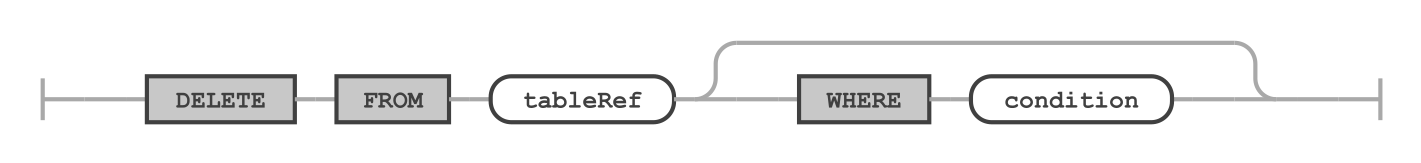
\includegraphics[width=\textwidth]{figures/deleteStmt.png}
	\caption{A \texttt{deleteStmt} grammatikai szabály railroad diagramja}
	\label{fig:rr_deletestmt}
\end{figure}

A \texttt{DELETE} utasítás fordítása az EF Core 8.0-ban bevezetett \\\texttt{ExecuteDeleteAsync()} metódusra épül. Ez a metódus közvetlenül az adatbázison hajt végre törlési műveletet, megkerülve az EF Core change trackert, ami azt jelenti, hogy nem szükséges az érintett entitásokat előbb a memóriába tölteni, majd törölni.

A fordítás alapesete a WHERE feltétel nélküli törlés, ahol a teljes tábla tartalma törlésre kerül (\ref{lst:delete_alap}. kódpélda).

\begin{lstlisting}[caption={DELETE WHERE feltétel nélkül}, label={lst:delete_alap}]
	// SQL: DELETE FROM Users
	// Generált LINQ:
	db.Users.ExecuteDeleteAsync()
\end{lstlisting}

WHERE feltétel esetén a lánc egy \texttt{Where()} hívással egészül ki, amelybe a feltétel ugyanazzal a scope-kezelési mechanizmussal kerül, mint a \texttt{SELECT} esetén. Ez lehetővé teszi, hogy korrelált allekérdezések is megjelenjenek a \texttt{DELETE} feltételében, ahogy azt \aref{lst:delete_korrelalt}. kódpélda mutatja.

\begin{lstlisting}[caption={DELETE korrelált allekérdezéssel}, label={lst:delete_korrelalt}]
	// SQL: DELETE FROM Users u WHERE EXISTS
	//        (SELECT 1 FROM Orders o WHERE o.Owner = u.Id)
	// Generált LINQ:
	db.Users.Where(x => (db.Orders.Where(o => o.Owner == x.Id)).Any())
	.ExecuteDeleteAsync()
\end{lstlisting}

A \texttt{DELETE} implementációja a \texttt{SetupTableScope} és \texttt{BuildWhereMethod} segédmetódusokat újrahasználja, amelyek a \texttt{SELECT} feldolgozásához készültek. Ez jól szemlélteti a háromrétegű architektúra előnyét, mivel az új utasítástípus bevezetésekor a WHERE-kezelési logikát nem kellett újraírni.

\Section{Az INSERT fordítása}

Az alfejezetben az \texttt{INSERT} utasítások fordítási módja kerül részletezésre.

\begin{figure}[H]
	\centering
	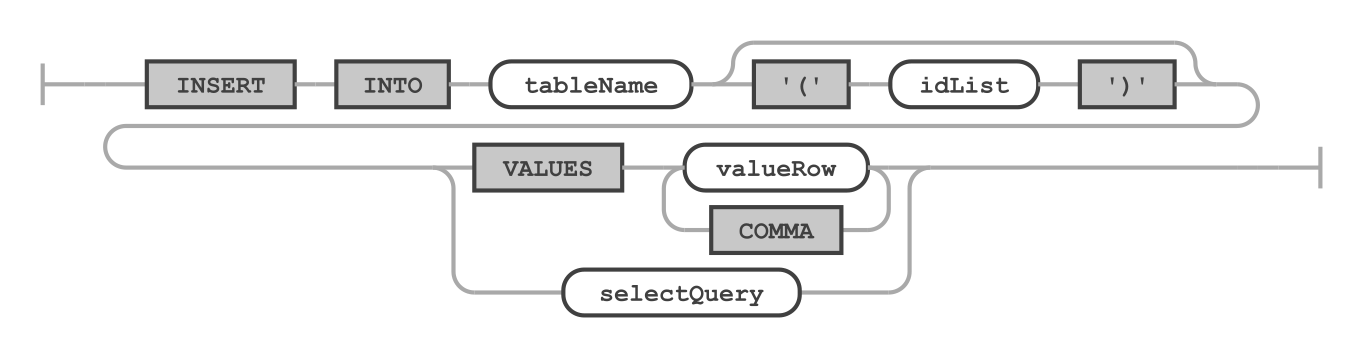
\includegraphics[width=\textwidth]{figures/insertStmt.png}
	\caption{Az \texttt{insertStmt} grammatikai szabály railroad diagramja}
	\label{fig:rr_insertstmt}
\end{figure}

Az \texttt{INSERT} utasítás két alakban támogatott. Az első a \texttt{VALUES} alapú beszúrás, a második az \texttt{INSERT INTO ... SELECT} alak, amely egy lekérdezés eredményét szúrja be a céltáblába.

\SubSection{VALUES alapú INSERT}

Egyetlen sor beszúrásakor az \texttt{Add()} metódus generálódik, több sor esetén az \texttt{AddRange()} egy \texttt{List<T>} példánnyal. Mindkét esetben a generált kód egy \texttt{SaveChanges()} hívással zárul, amely az EF Core change trackeren keresztül véglegesíti a változásokat (\ref{lst:insert_values}. kódpélda).

\begin{lstlisting}[caption={VALUES alapú INSERT fordítása}, label={lst:insert_values}]
	// SQL: INSERT INTO Users (Name, Age, Role) VALUES ('Bob', 25, 'Admin')
	// Generált LINQ:
	db.Users.Add(new Users { Name = "Bob", Age = 25, Role = "Admin" });
	db.SaveChanges();
	
	// SQL: INSERT INTO Users (Name, Age) VALUES ('Bob', 25), ('Alice', 19)
	// Generált LINQ:
	db.Users.AddRange(new List<Users>
	{
		new Users { Name = "Bob", Age = 25 },
		new Users { Name = "Alice", Age = 19 }
	});
	db.SaveChanges();
\end{lstlisting}

A \texttt{NULL} értékek kezelése egyszerű, a generált kódban a \texttt{null} kulcsszó jelenik meg az adott property értékeként, ami az EF Core számára egyértelműen adatbázis-szintű \texttt{NULL}-t jelent.

\SubSection{INSERT INTO ... SELECT}

Ez az alak egy meglévő lekérdezés eredményét szúrja be a céltáblába. A fordítás során a SELECT lekérdezés AST-je a \texttt{LinqInsertSelectNode}-ba kerül, amely a kódgeneráláskor a SELECT projekciót újraírja a céltábla típusára mutató inicializátorrá (\ref{lst:insert_select}. kódpélda).

\begin{lstlisting}[caption={INSERT INTO ... SELECT fordítása}, label={lst:insert_select}]
	// SQL: INSERT INTO Orders (Owner, Item, Qty)
	//      SELECT Id, 'Default', 0 FROM Users WHERE Role = 'Admin'
	// Generált LINQ:
	db.Orders.AddRange(
	(db.Users.Where(x => x.Role == "Admin"))
	.Select(x => new Orders { Owner = x.Id, Item = "Default", Qty = 0 })
	.ToList()
	);
	db.SaveChanges();
\end{lstlisting}

A projekció újraírása AST szinten történik, nem szövegmanipulációval. A \\ \texttt{LinqInsertSelectNode} a SELECT lánc végéről eltávolítja a névtelen objektumot előállító \texttt{Select()} hívást, és helyette egy typed inicializátort generál, amelynek property-jei az INSERT oszloplistájából, értékei pedig a SELECT projekció kifejezéseiből származnak. Ez biztosítja, hogy literálok (\texttt{'Default'}), konstansok (\texttt{0}) és oszlophivatkozások (\texttt{x.Id}) egyaránt helyesen kerüljenek be a generált kódba.

\Section{Az UPDATE fordítása}

Az alfejezetben az \texttt{UPDATE} utasítások fordítási módja kerül részletezésre.

\begin{figure}[H]
	\centering
	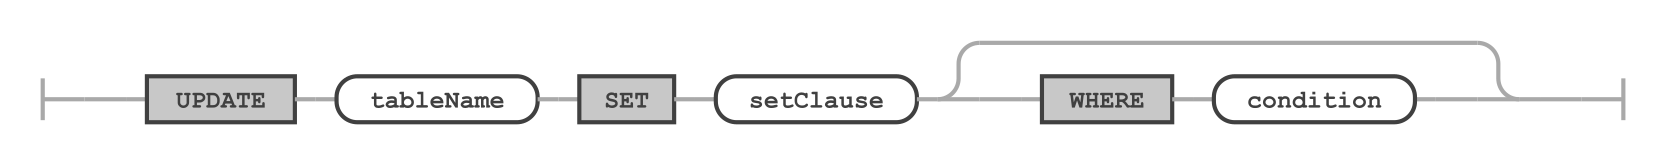
\includegraphics[width=\textwidth]{figures/updateStmt.png}
	\caption{Az \texttt{updateStmt} grammatikai szabály railroad diagramja}
	\label{fig:rr_updatestmt}
\end{figure}

Az \texttt{UPDATE} utasítás fordítása az EF Core 8.0-ban bevezetett \\\texttt{ExecuteUpdateAsync()} metódusra épül, amely a \texttt{ExecuteDeleteAsync()}-hoz hasonlóan közvetlenül az adatbázison hajt végre módosítást, a change tracker megkerülésével.

A \texttt{SET} záradék minden egyes értékadásából egy \texttt{.SetProperty()} hívás keletkezik, amelyek láncoltan kapcsolódnak egymáshoz. A \texttt{SetProperty()} két paramétert vár: az első egy lambda, amely azonosítja a módosítandó oszlopot, a második pedig az új értéket adja meg.

Az új érték megadásának alakja attól függ, hogy a jobb oldal tartalmaz-e oszlophivatkozást. Ha az értékadás jobb oldala kizárólag konstans (például \texttt{SET Role = 'Admin'}), a második argumentum direkt értékként jelenik meg. Ha azonban a jobb oldal hivatkozik az aktuális sorra (például \texttt{SET Points = Points + 10}), a második argumentum szintén lambda alakot ölt, amelynek törzsében az oszlophivatkozás a lambda paraméterével prefixelve szerepel. Mindkét esetet \aref{lst:update}. kódpélda szemlélteti.

\begin{lstlisting}[caption={UPDATE fordítása konstans és kifejezés értékkel}, label={lst:update}]
	// SQL: UPDATE Users SET Role = 'Admin' WHERE Age > 30
	// Generált LINQ:
	db.Users.Where(x => x.Age > 30).ExecuteUpdateAsync(s => s
	.SetProperty(x => x.Role, "Admin"))
	
	// SQL: UPDATE Users SET Points = Points + 10, Bonus = 0 WHERE Role = 'User'
	// Generált LINQ:
	db.Users.Where(x => x.Role == "User").ExecuteUpdateAsync(s => s
	.SetProperty(x => x.Points, x => x.Points + 10)
	.SetProperty(x => x.Bonus, 0))
\end{lstlisting}

A \texttt{NULL} értékre való frissítés külön kezelést igényel. A \texttt{SetProperty(x => x.Bonus,}\\ \texttt{null)} alak fordítási hibát okozna, mivel a fordítóprogram nem tudja inferálni a \texttt{null} típusát. A megoldás lambda alak alkalmazása: \\\texttt{SetProperty(x => x.Bonus, x => null)}, ahol az EF Core a bal oldali lambda visszatérési típusából (\texttt{int?}) következteti ki a \texttt{null} típusát.

A \texttt{SET} kifejezések látogatása ugyanazzal a \texttt{\_inWhereClause} flag mechanizmussal történik, mint a WHERE feltételeknél, így az oszlophivatkozások (\texttt{Points}, \texttt{Role}) helyesen kapják meg az \texttt{x.} prefixet a generált kódban.

\Section{A webes felület}

A fordító kipróbálásához egy Blazor WebAssembly alapú webes felület is készült. A Blazor WebAssembly a .NET alkalmazást a böngészőben, WebAssembly formában futtatja, így a fordító teljes egészében a felhasználó gépén működik, szerveroldali komponens nélkül. Az alkalmazás statikus weboldalként a GitHub Pages szolgáltatáson érhető el.

\Aref{fig:webes_felulet}. ábrán láthatunk illusztrációként egy képet a webes alkalmazás kinézetéről.
A felület két egymás melletti szerkesztőmezőből áll: a bal oldaliba az SQL utasítás kerül, a jobb oldaliban a generált LINQ kód jelenik meg. A fordítás egy gombnyomással indul, az eredmény a vágólapra másolható, és egy beépített példa egy \texttt{JOIN}, \texttt{GROUP BY} és \texttt{HAVING} záradékot is tartalmazó lekérdezést tölt be. A felület kijelzi a fordítás idejét, hiba esetén pedig a fordító kivételének üzenetét mutatja, így a nem támogatott konstrukciók is azonnal azonosíthatók. A fordítás eredménye mellett a felület két fát is meg tud jeleníteni, az ANTLR által előállított parse fát és a visitor által felépített köztes fát. Mindkettőt a fordító DOT formátumban adja át, a böngészőben pedig grafikus formában rajzolódnak ki, így a fordítás menete a bemenettől a generált kódig vizuálisan is követhető. A felület magyar és angol nyelven is használható.

\begin{figure}[H]
	\centering
	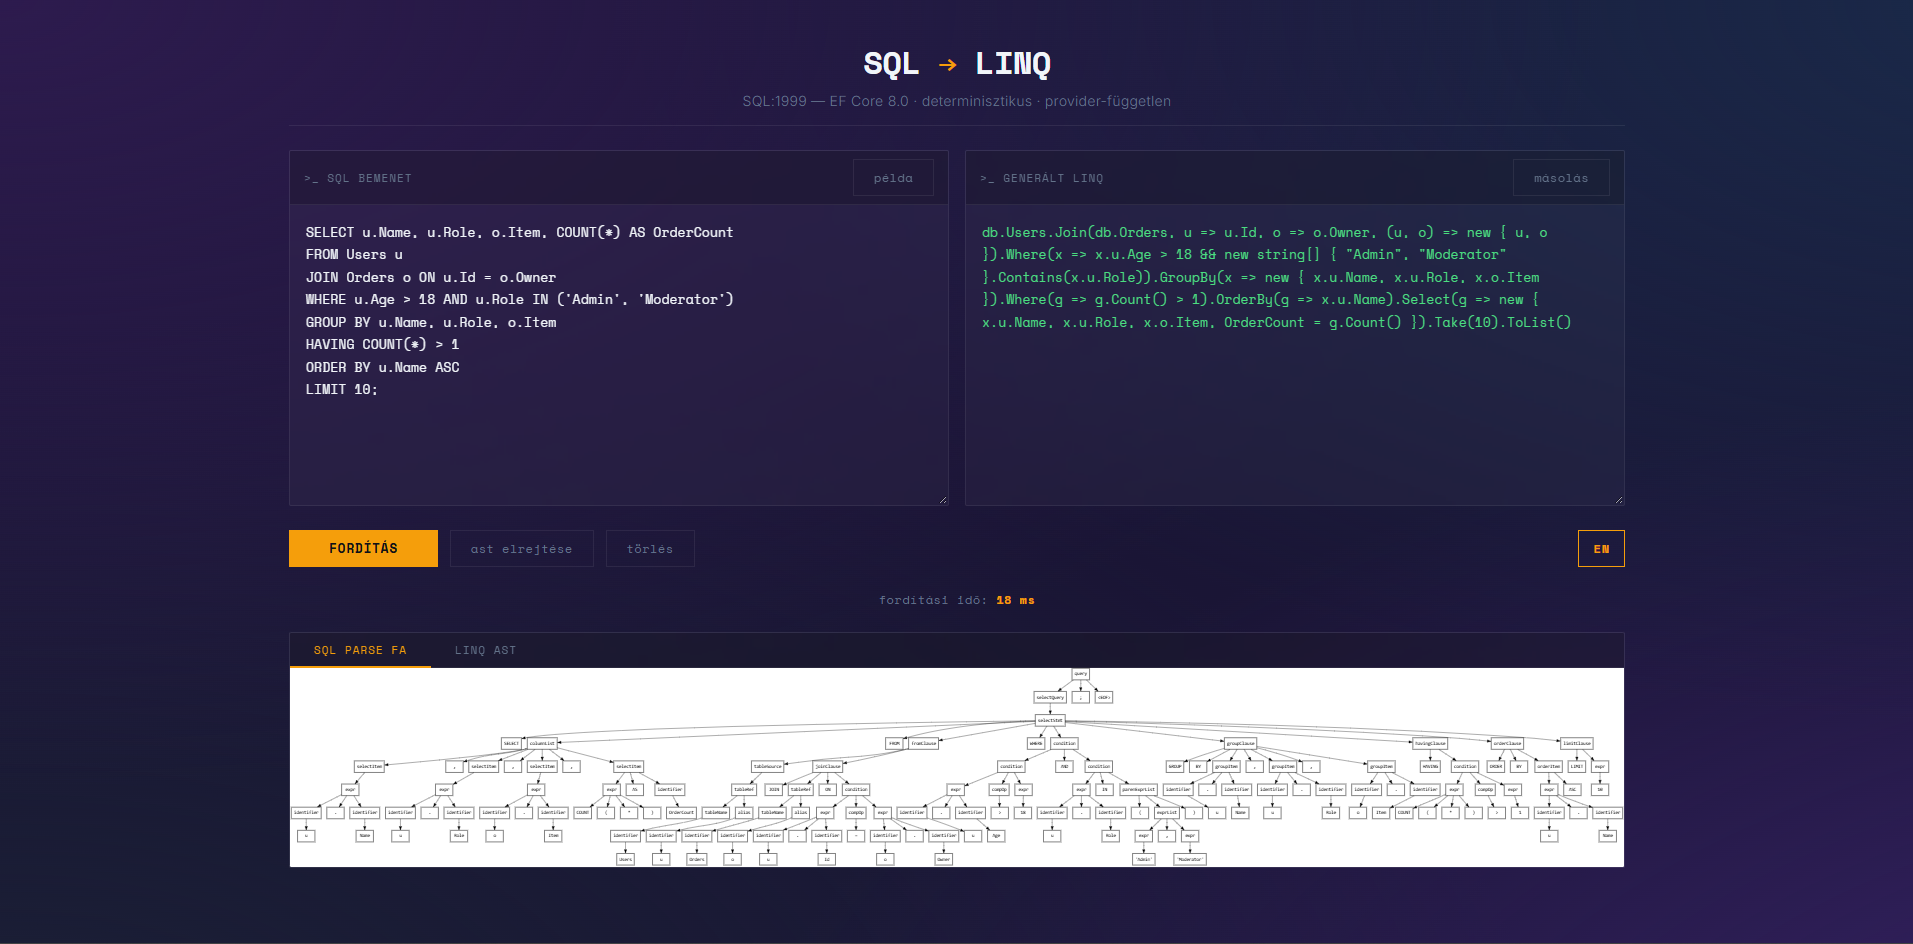
\includegraphics[width=\textwidth]{figures/webes_felulet.png}
	\caption{A webes felület egy lefordított lekérdezéssel}
	\label{fig:webes_felulet}
\end{figure}

\Chapter{Tesztelés}
\label{chap:teszteles}

A fordító helyességének igazolása három egymást kiegészítő tesztelési szinten történik. Az első szintet a string-szintű transpiler tesztek alkotják, amelyek a generált kódot elvárt kimenetekkel vetik össze. A második szint a szemantikai ekvivalencia teszteké, amelyek a generált kódot ténylegesen lefuttatják, és az eredményét az eredeti SQL eredményével hasonlítják össze. A harmadik szintet a fuzz tesztek jelentik, amelyek véletlenszerűen generált utasításokon vizsgálják a fordító robusztusságát. Mindhárom szint más-más típusú hibát képes felderíteni, és együttesen lefedik a fordítás teljes folyamatát a szintaktikai elemzéstől a szemantikai egyenértékűségig. A tesztelési infrastruktúra felépítését \aref{fig:pipeline_teszteles}. ábra mutatja.

A tesztosztályok és a bennük található tesztek számát \aref{tab:tesztek}. táblázat foglalja össze.

\begin{table}[H]
	\centering
	\renewcommand{\arraystretch}{1.4}
	\small
	\begin{tabularx}{\textwidth}{|>{\raggedright\arraybackslash}p{0.36\textwidth}|>{\raggedright\arraybackslash}p{0.15\textwidth}|>{\centering\arraybackslash}p{0.11\textwidth}|>{\raggedright\arraybackslash}X|}
		\hline
		\textbf{Tesztosztály} & \textbf{Szint} & \textbf{Tesztek} & \textbf{Megjegyzés} \\
		\hline
		\texttt{TranspilerTests} & string-szintű & 267 & \texttt{IOPairs.json} alapján \\
		\hline
		\texttt{ErrorPathTests} & string-szintű & 30 & hibaágak, kivételtípusok \\
		\hline
		\texttt{PascalCaseTests} & string-szintű & 5 & névkonverzió \\
		\hline
		\texttt{SemanticEquivalenceTests} & szemantikai & 267 + 1 & 190 futó, 77 kizárt eset, 1 fuzz teszt \\
		\hline
		\texttt{EfCoreEdgeCaseTests} & szemantikai & 80 & EF Core fordítás, DML \\
		\hline
		\texttt{OuterJoinSemanticTests} & szemantikai & 13 & outer join, külön séma \\
		\hline
		\texttt{FuzzTests} & fuzz & 2 & 2500 \texttt{SELECT} és 3000 DML iteráció \\
		\hline
	\end{tabularx}
	\caption{A tesztosztályok összesítése}
	\label{tab:tesztek}
\end{table}

\begin{figure}[H]
	\centering
	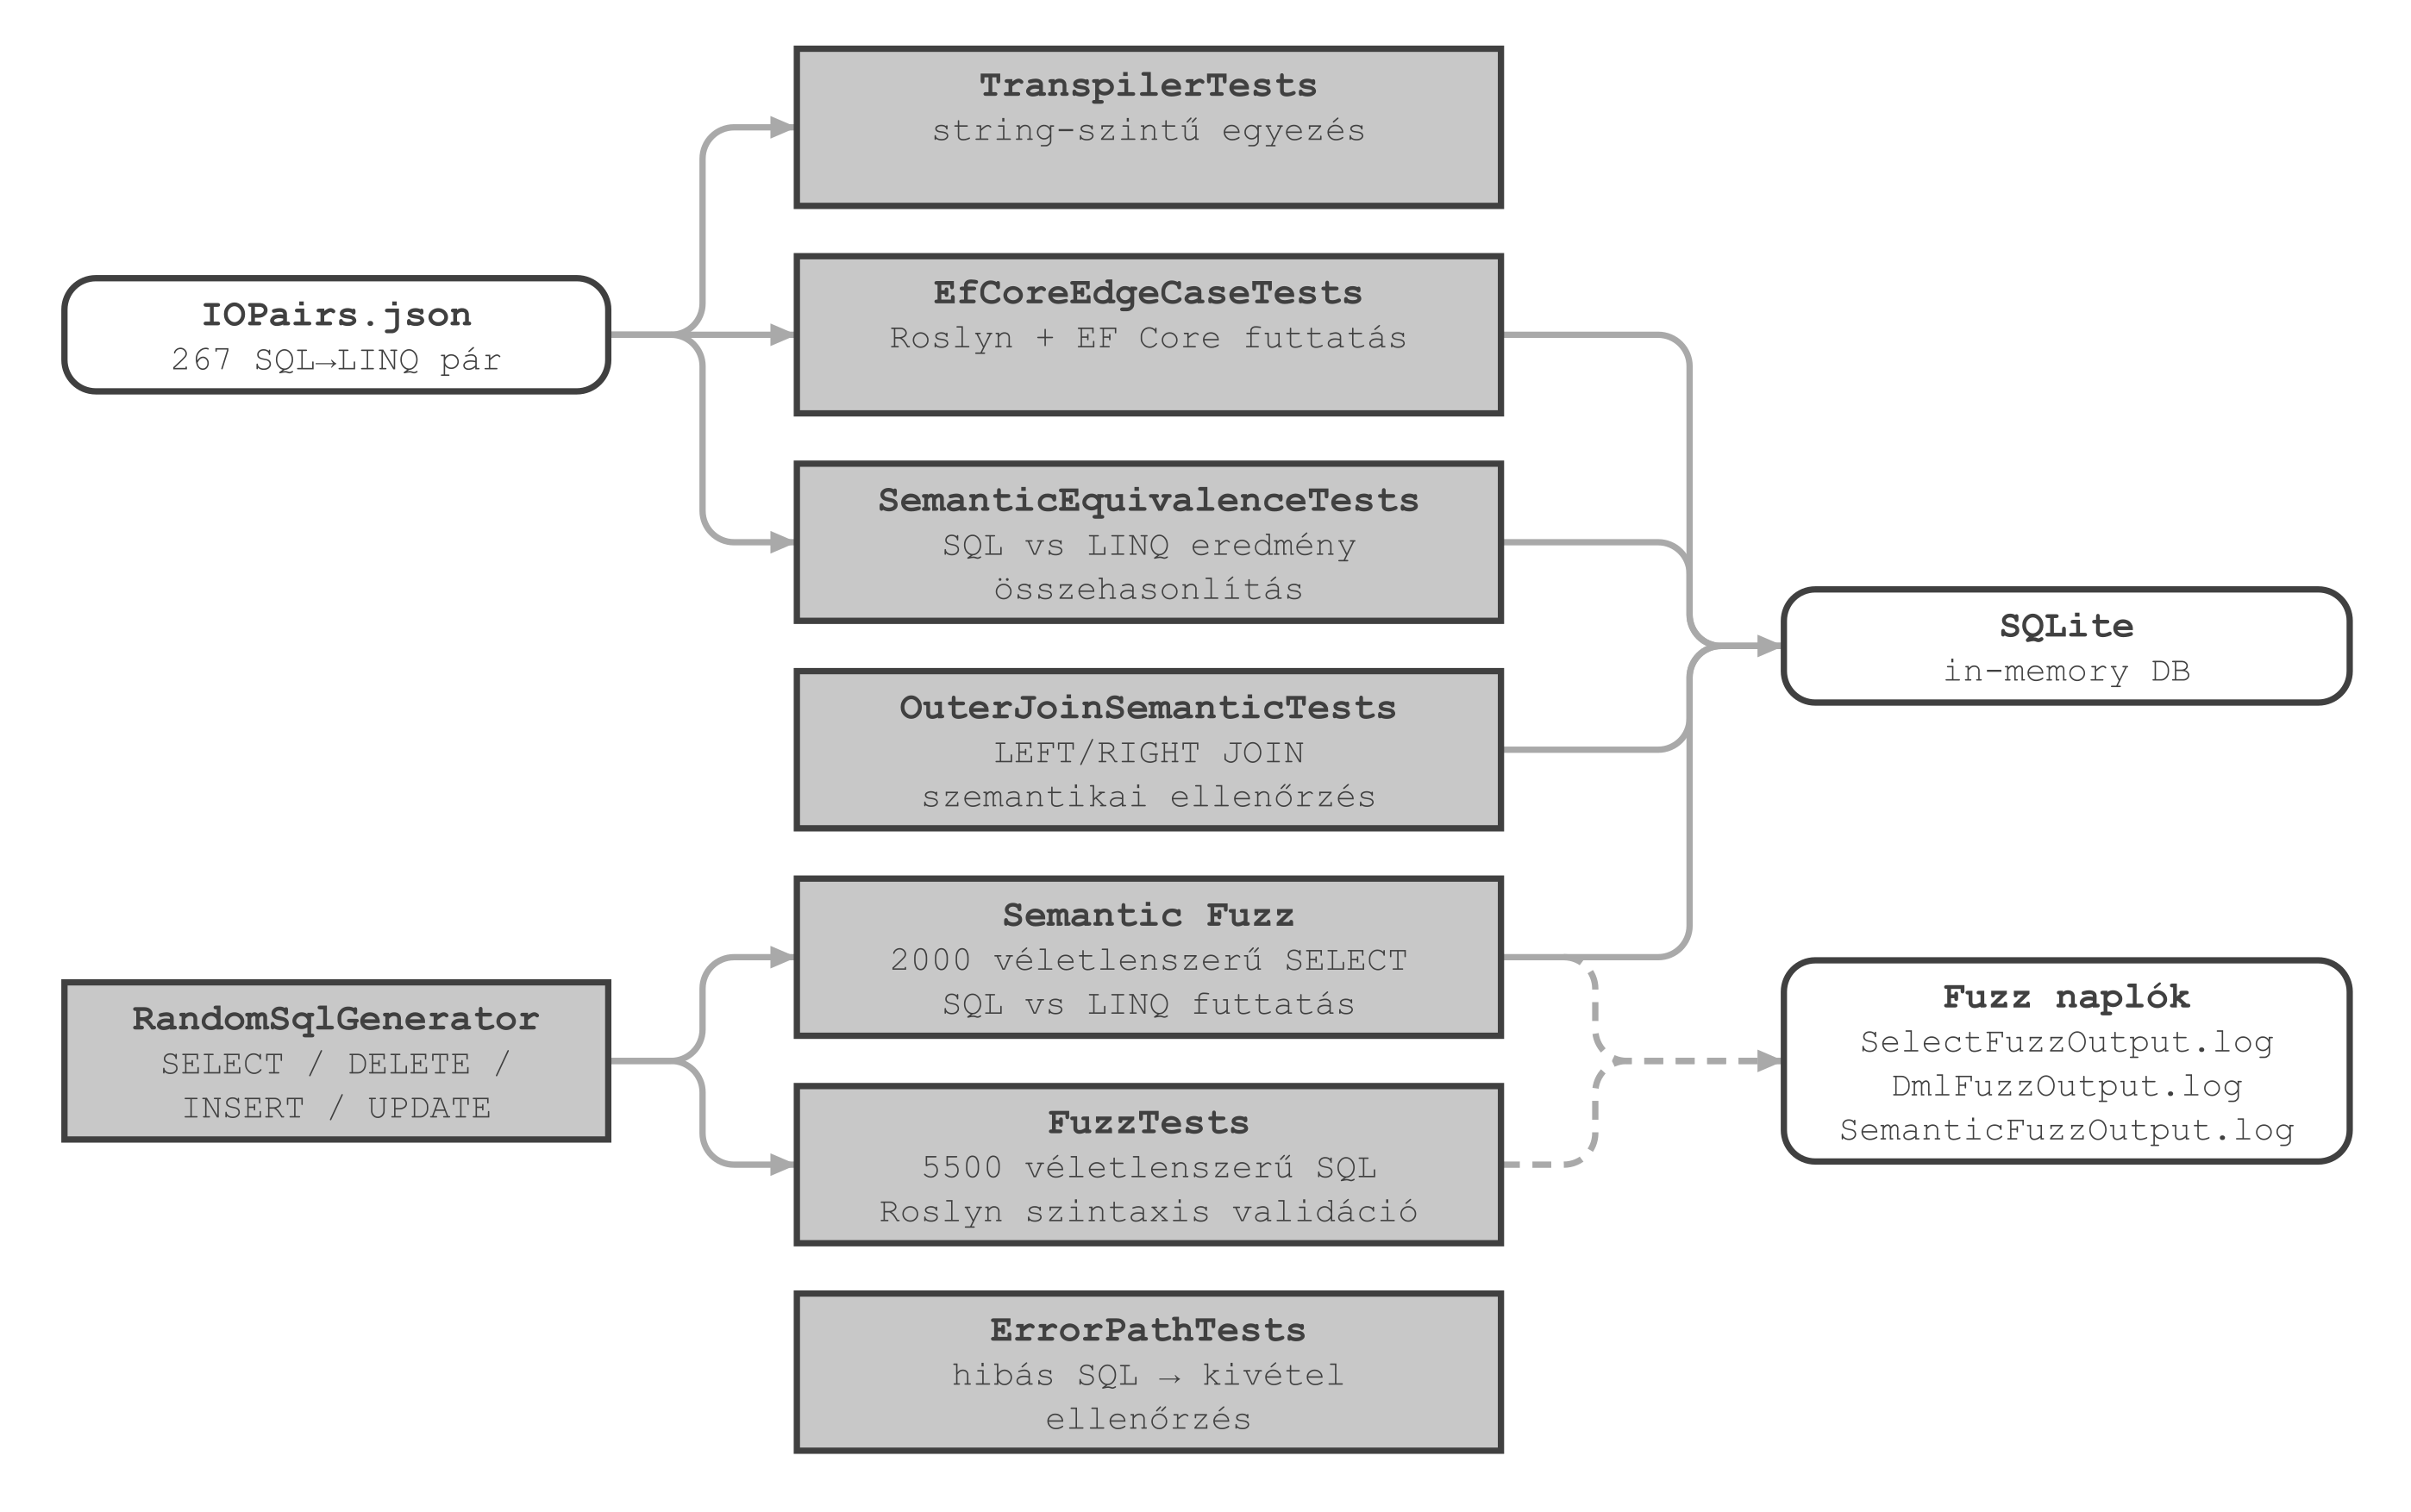
\includegraphics[width=\textwidth]{figures/pipeline_teszteles.png}
	\caption{A tesztelési infrastruktúra felépítése}
	\label{fig:pipeline_teszteles}
\end{figure}

A tesztek az NUnit keretrendszerre épülnek, és a .NET parancssori eszközével vagy a Visual Studio Test Explorer ablakából futtathatók. A teljes tesztkészletet a megoldás gyökérmappájában kiadott \texttt{dotnet test} parancs futtatja le, egy tesztosztály pedig a \texttt{-{}-filter} kapcsolóval külön is futtatható. Az alábbi példa első sora a teljes tesztkészletet, a második csak a szemantikai teszteket futtatja.

\begin{lstlisting}[language={}]
dotnet test
dotnet test --filter "FullyQualifiedName~SemanticEquivalenceTests"
\end{lstlisting}

A tesztek forráskódja a projekt repójának \texttt{SqlToLinq.Tests} mappájában érhető el. A fuzz tesztek naplófájljai a tesztek munkakönyvtárába, alapértelmezés szerint a tesztprojekt kimeneti mappájába kerülnek, a pontos útvonalat a tesztek futás közben ki is írják.

\Section{Transpiler tesztek}

A legegyszerűbb és leggyorsabb tesztelési szint az \texttt{IOPairs.json} fájlban tárolt SQL→LINQ párok string-szintű összehasonlítása. A fájl 267 tesztesetet tartalmaz, amelyek minden támogatott SQL konstrukciót lefednek, az egyszerű \texttt{SELECT} lekérdezésektől a háromtáblás JOIN-okon, korrelált allekérdezéseken és \texttt{GROUP BY} aggregátumokon át a DML utasításokig.

A \texttt{TranspilerTests} osztály minden tesztesethez meghívja \\az \texttt{SqlToLinqConverter.Convert()} metódust, majd a generált és az elvárt LINQ kódot szóközök eltávolítása után hasonlítja össze. Ez a normalizálás szükséges, mert a fordító nem garantál egzakt szöveg szintű (\textit{whitespace}) formázást, csak a kód szerkezetével foglalkozik. Ha az összehasonlítás sikertelen, a hibaüzenet tartalmazza a bemeneti SQL-t, a generált és az elvárt kimenetet, megkönnyítve a regresszió azonosítását.

A tesztek egy különálló \texttt{ErrorPathTests} osztályba is szerveződnek, amelyek azt ellenőrzik, hogy a fordító a megfelelő kivételt dobja érvénytelen vagy nem támogatott bemenet esetén. Ez magában foglalja a lexer- és parser-szintű szintaktikai hibákat (\texttt{SqlSyntaxException}), a nem fordítható SQL konstrukciókat (\texttt{NotSupportedException}), az ismeretlen függvényneveket, a helytelen argumentumszámot és a típusrendszerből fakadó korlátokat, például a string típusú oszlopokra alkalmazott összehasonlító operátorokat.

\Section{Szemantikai ekvivalencia tesztek}

A string-szintű egyezés elégséges, de nem szükséges feltétele a helyességnek. Egy generált LINQ lekérdezés lehet szintaktikailag helyes, mégis különböző eredményt adhat mint az eredeti SQL. A \texttt{SemanticEquivalenceTests} osztály ezért egy lépéssel tovább megy, mind a bemeneti SQL-t, mind a belőle generált LINQ kódot ténylegesen lefuttatja egy SQLite in-memory adatbázison, és az eredményhalmazokat hasonlítja össze.

A végrehajtás a Microsoft Roslyn fordítóplatform segítségével történik. A generált LINQ kódot a tesztelési infrastruktúra dinamikusan C\# forráskóddá formázza, majd a \\ \texttt{CSharpCompilation} osztállyal memóriában lefordítja és futtatja. Ez a megközelítés lehetővé teszi, hogy a tesztek ne csak a fordító kimenetét ellenőrizzék, hanem annak tényleges futási eredményét is, minden további kézzel írt kód nélkül. Ha a Roslyn fordítás sikertelen, a hibaüzenet tartalmazza a generált forráskódot és az összes fordítási hibát, ami megkönnyíti a diagnosztikát.

A tesztek determinisztikusak és reprodukálhatóak. Az adatbázist minden teszt előtt ugyanazok a kézzel összeállított adatok töltik fel, hat felhasználó, valamint a hozzájuk kapcsolódó rendelések, termékek, kategóriák és raktárak. Az adatok úgy lettek összeállítva, hogy a táblák között egymással JOIN-kapcsolatban álló és pár nélküli sorok is legyenek, például vannak rendelés nélküli felhasználók. Az outer joinok mindkét oldali illeszkedés nélküli sorainak ellenőrzése egy külön tesztosztályban, saját adatkészlettel történik. Az eredmény-összehasonlítás sor szintű, az ORDER BY záradék nélküli lekérdezéseknél a sorok sorba rendezés után, rendezéssel rendelkezőknél eredeti sorrendben kerülnek összevetésre.

Bizonyos teszteseteket ki kellett zárni ebből a szintből. A 267 esetből 80 nem fut le szemantikai összevetéssel, a kizárásnak pedig három fő oka van.

\begin{itemize}
	\item Az első a dialektusfüggő függvények köre. Az SQLite nem tartalmaz minden SQL Server, MySQL vagy Oracle specifikus függvényt, így a \texttt{YEAR()}, \texttt{MONTH()}, \texttt{DATEADD()}, \texttt{DATEDIFF()}, \texttt{GETDATE()} és hasonló dátumfüggvények, valamint a \texttt{LEN()}, \texttt{ISNULL()}, \texttt{NVL()}, \texttt{STUFF()} és rokon szöveg- és matematikai függvények nyers SQL-ként nem futtathatók.
	\item A második ok a logikai literálok eltérő kezelése, mivel az SQLite a \texttt{TRUE} és \texttt{FALSE} értékeket egész számként adja vissza, míg a generált LINQ \texttt{bool} típusú eredményt állít elő.
	\item A harmadik csoportot a \texttt{DELETE}, \texttt{INSERT} és \texttt{UPDATE} utasítások alkotják (összesen 28 eset), amelyek nem eredményhalmazt adnak vissza, hanem az adatbázis állapotát módosítják, ezért ezek ellenőrzése külön, az \texttt{EfCoreEdgeCaseTests} osztályban történik.
\end{itemize}

A kizárt eseteket egy explicit kizárási lista alapján az \texttt{Assert.Ignore()} hívással átugorja a rendszer, a helyességüket pedig a transpiler tesztek biztosítják. A fennmaradó 187 eset esetében a nyers SQL és a generált LINQ eredményhalmaza ténylegesen összevetésre kerül.

A \texttt{DELETE}, \texttt{INSERT} és \texttt{UPDATE} utasítások szemantikai ellenőrzése külön \\ \texttt{EfCoreEdgeCaseTests} osztályban történik. Ezek a tesztek ténylegesen módosítják az adatbázist, majd az EF Core \texttt{DbContext}-en keresztül ellenőrzi az adatbázis állapotát. Mivel a módosítások megváltoztatják a seed adatokat, minden teszt esetén a \texttt{[SetUp]} metódus újra feltölti az adatbázist. A \texttt{NULL} értékre való \texttt{UPDATE} esetén külön figyelmet igényel az EF Core type inference, mivel a \texttt{SetProperty(x => x.Col, null)} alak fordítási hibát okoz, mert a fordítóprogram nem tudja inferálni a \texttt{null} típusát, ezért a generált kód \texttt{SetProperty(x => x.Col, x => null)} alakot használ, ahol a bal oldali lambda visszatérési típusából az EF Core következteti ki a megfelelő nullable típust.

Az outer join szemantika tesztelése egy külön \texttt{OuterJoinSemanticTests} osztályban történik, dedikált \texttt{OuterJoinDbContext}-tel és seed adatokkal. A seed adatok szándékosan tartalmaznak illeszkedés nélküli sorokat mindkét oldalon, a \texttt{Customers} táblában vannak rendelés nélküli vásárlók, az \texttt{Invoices} táblában pedig nem létező vásárlóra hivatkozó számlák. Ez teszi lehetővé, hogy a \texttt{LEFT JOIN} által megőrzött bal oldali és a \texttt{RIGHT JOIN} által megőrzött jobb oldali sorok viselkedése egyaránt ellenőrizhető legyen.

\Section{Fuzz tesztek}

A fuzz tesztelés a fordító robusztusságát vizsgálja véletlenszerűen generált, de grammatikailag érvényes SQL lekérdezéseken. A módszer Miller és társai \cite{miller1990fuzz} munkájából ered, akik véletlenszerű bemenetekkel a UNIX segédprogramok jelentős részét hibás működésre tudták bírni. Fordítóprogramok és adatbázis-kezelők tesztelésénél a teljesen véletlen karaktersorozatok helyett jellemzően a bemeneti nyelv szerkezetét követő, generált bemeneteket használnak, mert a véletlen szöveget már a lexer elutasítaná. Slutz \cite{slutz1998rags} például véletlenszerű, de szintaktikailag helyes SQL lekérdezéseket generált, és ezek eredményét több adatbázis-kezelő között vetette össze. A jelen munka szemantikai fuzz tesztje ugyanezt az elvet követi, azzal a különbséggel, hogy az összevetés a nyers SQL és a generált LINQ eredményhalmaza között történik.

A \texttt{RandomSqlGenerator} osztály egy rögzített maggal (seed) inicializált véletlenszám-generátor segítségével állít elő SQL utasításokat, amelyek lefedik a fordító összes főbb ágát.

A \texttt{FuzzTests} osztály két tesztet tartalmaz. Az első 2500 véletlenszerű \texttt{SELECT} lekérdezést fordít le és ellenőrzi a generált C\# kód szintaktikai helyességét a Roslyn \\ \texttt{SyntaxFactory.ParseExpression()} metódusával. A második 3000 DML utasítást generál egyenlő arányban \texttt{DELETE}, \texttt{INSERT} és \texttt{UPDATE} között, és a generált kódot \\ \texttt{CSharpSyntaxTree.ParseText()} segítségével validálja, mivel a DML kimenet statement, nem kifejezés. Mindkét teszt logfájlba írja az eredményeket (\texttt{SelectFuzzOutput.log}, \texttt{DmlFuzzOutput.log}), amelyek \texttt{[PASS]}, \texttt{[SKIP]} és \texttt{[FAIL]} bejegyzéseket tartalmaznak.

A \texttt{NotSupportedException}-nel záruló eseteket a fuzz tesztek \texttt{[SKIP]}-ként kezelik, ezek olyan véletlenszerűen generált kombinációk, amelyek egyébként érvényes SQL-t alkotnak, de a fordító nem támogatja őket (például string típusú oszlopra alkalmazott \texttt{BETWEEN} operátor). Ezt a viselkedést az \texttt{ErrorPathTests} osztály explicit tesztesetei ellenőrzik.

A \texttt{SemanticEquivalenceTests} osztály szintén tartalmaz egy fuzz alapú szemantikai tesztet, amely 2000 véletlenszerű \texttt{SELECT} lekérdezést fordít le, majd mind a nyers SQL-t, mind a generált LINQ-ot lefuttatja az SQLite adatbázison, és az eredményhalmazokat összehasonlítja. Ez a teszt a legkörülményesebb, de egyben a legerősebb biztosíték, mivel ha itt sikeres, az azt jelenti, hogy a fordítás nem csupán szintaktikailag helyes kódot állít elő, hanem szemantikailag ekvivalens lekérdezést is.

Az iterációk száma a lefedettség és a futási idő közötti kompromisszum eredménye. Minden iteráció egy teljes Roslyn-fordítást és két adatbázis-lekérdezést tartalmaz, ezért ez a teszt nagyságrendekkel lassabb, mint a csak szintaktikai ellenőrzést végző fuzz tesztek. 2000 iteráció mellett a teszt körülbelül \textbf{5} perc alatt fut le, ami még belefér egy fejlesztési ciklusba, és a generátor ennyi iteráció alatt az általa előállítható összes lekérdezésszerkezetet (egy-, két- és háromtáblás lekérdezések, allekérdezések, csoportosítás, inline nézetek) többször is előállítja. A rögzített seed miatt a lefuttatott lekérdezések köre minden futtatásnál azonos, így egy esetleges hiba mindig reprodukálható.

\Chapter{LLM összehasonlítás}
\label{chap:llm}

A nagy nyelvi modellek (Large Language Model, röviden LLM) hatalmas szöveggyűjteményeken előtanított neurális hálózatok, amelyek a választ a bemeneti szöveg folytatásaként, tokenről tokenre építik fel. Brown és társai \cite{brown2020gpt3} megmutatták, hogy kellően nagy modellek külön tanítás nélkül, néhány példa vagy egy szöveges utasítás alapján is képesek új feladatok megoldására. Chen és társai \cite{chen2021codex} a forráskódon tovább tanított modellek programozási képességeit vizsgálták, és azt találták, hogy ezek természetes nyelvű leírásból a feladatok egy részében működő kódot állítanak elő, a helyesség azonban nem garantált, ezért a generált kódot ellenőrizni kell. A kimenet nemdeterminisztikus jellege külön vizsgálatok tárgya. Ouyang és társai \cite{ouyang2025nondeterminism} a ChatGPT kódgenerálását vizsgálva azt tapasztalták, hogy ugyanarra a feladatra adott válaszok futtatásonként jelentősen eltérhetnek egymástól, amelyet a mintavételi hőmérséklet nullára állítása csökkent némiképp, de nem szüntet meg teljesen.

A projekt egyik motivációja az volt, hogy az LLM-ek ugyan képesek SQL lekérdezéseket LINQ kóddá alakítani, de ez a folyamat statisztikai alapú, nem determinisztikus, így fenntartásokkal integrálható automatizált pipeline-ba. Ennek empirikus vizsgálatára méréseket végeztem, amelyek során három LLM válaszidejét, kimenetének állandóságát és helyességét, valamint a mérés költségét vizsgáltam ugyanazokon a bemeneteken.

\Section{Módszertan}

A mérés bemenete öt, egyre összetettebb SQL lekérdezés (Q1--Q5), amelyek a fordító által támogatott nyelvi elemek egy-egy jellemző kombinációját fedik le. A Q1 egyszerű szűrést és rendezést tartalmaz. A Q2 csoportosít, \texttt{HAVING} feltétellel szűri a csoportokat, és az aggregátum aliasára rendez. A Q3 egy kéttáblás \texttt{LEFT JOIN} szűréssel, rendezéssel és \texttt{LIMIT} záradékkal. A Q4 egy \texttt{CASE WHEN} kifejezést és egy korrelált \texttt{EXISTS} allekérdezést tartalmaz. A Q5 három táblát kapcsol össze, és egy \texttt{LIKE} mintát, zárójelezett összetett feltételt, valamint \texttt{LIMIT} és \texttt{OFFSET} záradékot is tartalmaz. A lekérdezések teljes szövege és a modelleknek küldött prompt a mellékletben megtalálható.

A három vizsgált modell a Google Gemini 3.6 Flash és Gemini 4 Argon modellje, valamint az OpenAI nyílt súlyú GPT-OSS-120B modellje volt, utóbbi a Groq infrastruktúráján futtatva. A Gemini 3.6 Flash egy gyors, olcsóbb modell, a Gemini 4 Argon a Google nagyobb, drágább modellje. Mindhárom modell a válasz előtt belső gondolatmenetet (reasoning) állít elő, amely a válaszban nem jelenik meg, de a válaszidőbe és a költségbe beleszámít.

Minden modell ugyanazt a promptot kapta, amely kizárólag a LINQ kifejezést kérte vissza, magyarázat és formázás nélkül. A hívások 0 hőmérséklettel és 16384 tokenes kimeneti korláttal futottak. A magas korlát azt biztosította, hogy a gondolatmenet ne vágja le a választ. Minden modell minden lekérdezésre 10 választ adott, így összesen 150 hívás történt. A futtatások két, egyenként 5 futtatásos batchben, 2026. október 27-én délelőtt , illetbe délután, az esti órákban zajlottak, hogy a felhőszolgáltatások napszakonként eltérő terheltsége is megjelenjen az adatokban. Egy batchen belül a modellek és a lekérdezések hívásai felváltva követték egymást, két hívás között 5 másodperc szünettel, így mindhárom modell hasonló hálózati körülmények között válaszolt.

A mérést egy Python szkript végezte, amely a modellek nyilvános API-ját streamelt hívással érte el, és \texttt{time.perf\_counter()} segítségével rögzítette a kérés elküldésétől az első kimeneti token, illetve a teljes válasz megérkezéséig eltelt időt.    Minden hívás minden adata, a válaszidők, a kimenet, a leállás oka és a tokenszámok, fájlba került, így a kiértékelés a nyers adatokból bármikor megismételhető.

A kimeneteket három szempont szerint értékeltem. Először a futtatások kimeneteit vetettem össze egymással a transpiler teszteknél is alkalmazott normalizálással, a szóközök eltávolítása után. Ez a mérőszám a formázási eltéréseket kiszűri, de az eltérő változónév már különbségnek számít. Mivel a modellek a \texttt{DbContext} változót futtatásonként másként nevezték el, egy második mérőszám ettől és a záró pontosvesszőtől is eltekint, így csak a lekérdezés szerkezetét hasonlítja össze. Másodszor minden egyedi kimenetet kézzel ellenőriztem, hogy lefordítható-e, és ugyanazt az eredményt adja-e, mint az eredeti SQL lekérdezés. Harmadszor a leállás oka alapján azt vizsgáltam, hogy a kimenet teljes-e, vagyis nem üres és nem szakad-e meg.

Az LLM-mérések hálózati kéréseket tartalmaznak. A rögzített válaszidő magában foglalja a hálózati késleltetést, a szerver oldali sorban állást és feldolgozást, valamint a streamelt válasz fogadását, így a mért értékek nem csupán a modell sebességét tükrözik, hanem a felhőszolgáltatás pillanatnyi állapotát is. A saját fordító ebben a mérésben nem szerepel külön sorként. Lokálisan, hálózati kérés nélkül fut, a kimenete pedig determinisztikus, így ugyanarra a lekérdezésre minden futtatásnál ugyanazt a kódot adja, amit a tesztkészlet is igazol.

\Section{Eredmények}

\Aref{tab:llm-comparison}. táblázat lekérdezésenként foglalja össze a válaszidőket és a kimenetek változatosságát. Az első token oszlop azt az időt mutatja, amely a kérés elküldésétől a válasz első látható tokenjéig eltelt.

\begin{table}[H]
	\centering
	\renewcommand{\arraystretch}{1.3}
	\footnotesize
	\begin{tabular}{|c|r|r|r|r|r|c|c|}
		\hline
		\textbf{Lek.} & \textbf{Átlag} & \textbf{Szórás} & \textbf{Min} & \textbf{Max} & \textbf{Első token} & \textbf{Eltérő} & \textbf{Szerkezet} \\
		& \textbf{(s)} & \textbf{(s)} & \textbf{(s)} & \textbf{(s)} & \textbf{(s)} & & \\
		\hline
		\multicolumn{8}{|l|}{\textbf{Gemini 3.6 Flash}} \\
		\hline
		Q1 & 3,52 & 0,91 & 2,30 & 4,78 & 3,40 & 2 & 1 \\
		Q2 & 5,70 & 0,53 & 5,10 & 6,71 & 5,42 & 4 & 2 \\
		Q3 & 8,65 & 1,22 & 6,08 & 9,61 & 8,15 & 6 & 5 \\
		Q4 & 6,61 & 1,14 & 5,22 & 8,08 & 6,30 & 4 & 1 \\
		Q5 & 10,02 & 1,56 & 6,61 & 11,59 & 9,30 & 7 & 6 \\
		\hline
		\multicolumn{8}{|l|}{\textbf{Gemini 4 Argon}} \\
		\hline
		Q1 & 6,91 & 4,91 & 3,39 & 19,53 & 6,48 & 1 & 1 \\
		Q2 & 5,34 & 1,94 & 3,34 & 9,79 & 4,63 & 1 & 1 \\
		Q3 & 21,80 & 18,48 & 3,75 & 59,96 & 20,79 & 2 & 2 \\
		Q4 & 7,18 & 3,86 & 3,46 & 14,80 & 6,41 & 2 & 2 \\
		Q5 & 27,66 & 31,32 & 6,36 & 89,40 & 26,14 & 2 & 2 \\
		\hline
		\multicolumn{8}{|l|}{\textbf{GPT-OSS-120B (Groq)}} \\
		\hline
		Q1 & 0,88 & 0,17 & 0,62 & 1,15 & 0,79 & 2 & 1 \\
		Q2 & 0,83 & 0,13 & 0,64 & 1,08 & 0,69 & 2 & 1 \\
		Q3 & 1,54 & 0,15 & 1,32 & 1,79 & 1,31 & 2 & 2 \\
		Q4 & 1,18 & 0,26 & 0,91 & 1,82 & 1,04 & 2 & 1 \\
		Q5 & 1,57 & 0,18 & 1,13 & 1,75 & 1,26 & 2 & 2 \\
		\hline
	\end{tabular}
	\caption{A válaszidők és a kimenetek változatossága lekérdezésenként, 10 futtatás alapján. Az Eltérő oszlop a szóközök eltávolítása után különböző kimenetek számát, a Szerkezet oszlop a \texttt{DbContext} nevétől is eltekintve különböző kimenetek számát mutatja.}
	\label{tab:llm-comparison}
\end{table}

A válaszidők eloszlását \aref{fig:llm_hist_lekerdezes}. ábra lekérdezésenként, \aref{fig:llm_hist_osszesitett}. ábra modellenként összesítve mutatja. A válaszidők a GPT-OSS-120B egy-két másodperces és a Gemini 4 Argon akár másfél perces tartománya között mozognak, ezért a hisztogramok vízszintes tengelyének skálája panelenként eltér. Az ábrák összevetésekor a tengelyeken szereplő értékekre különösen figyelni kell.

\begin{figure}[h]
	\centering
	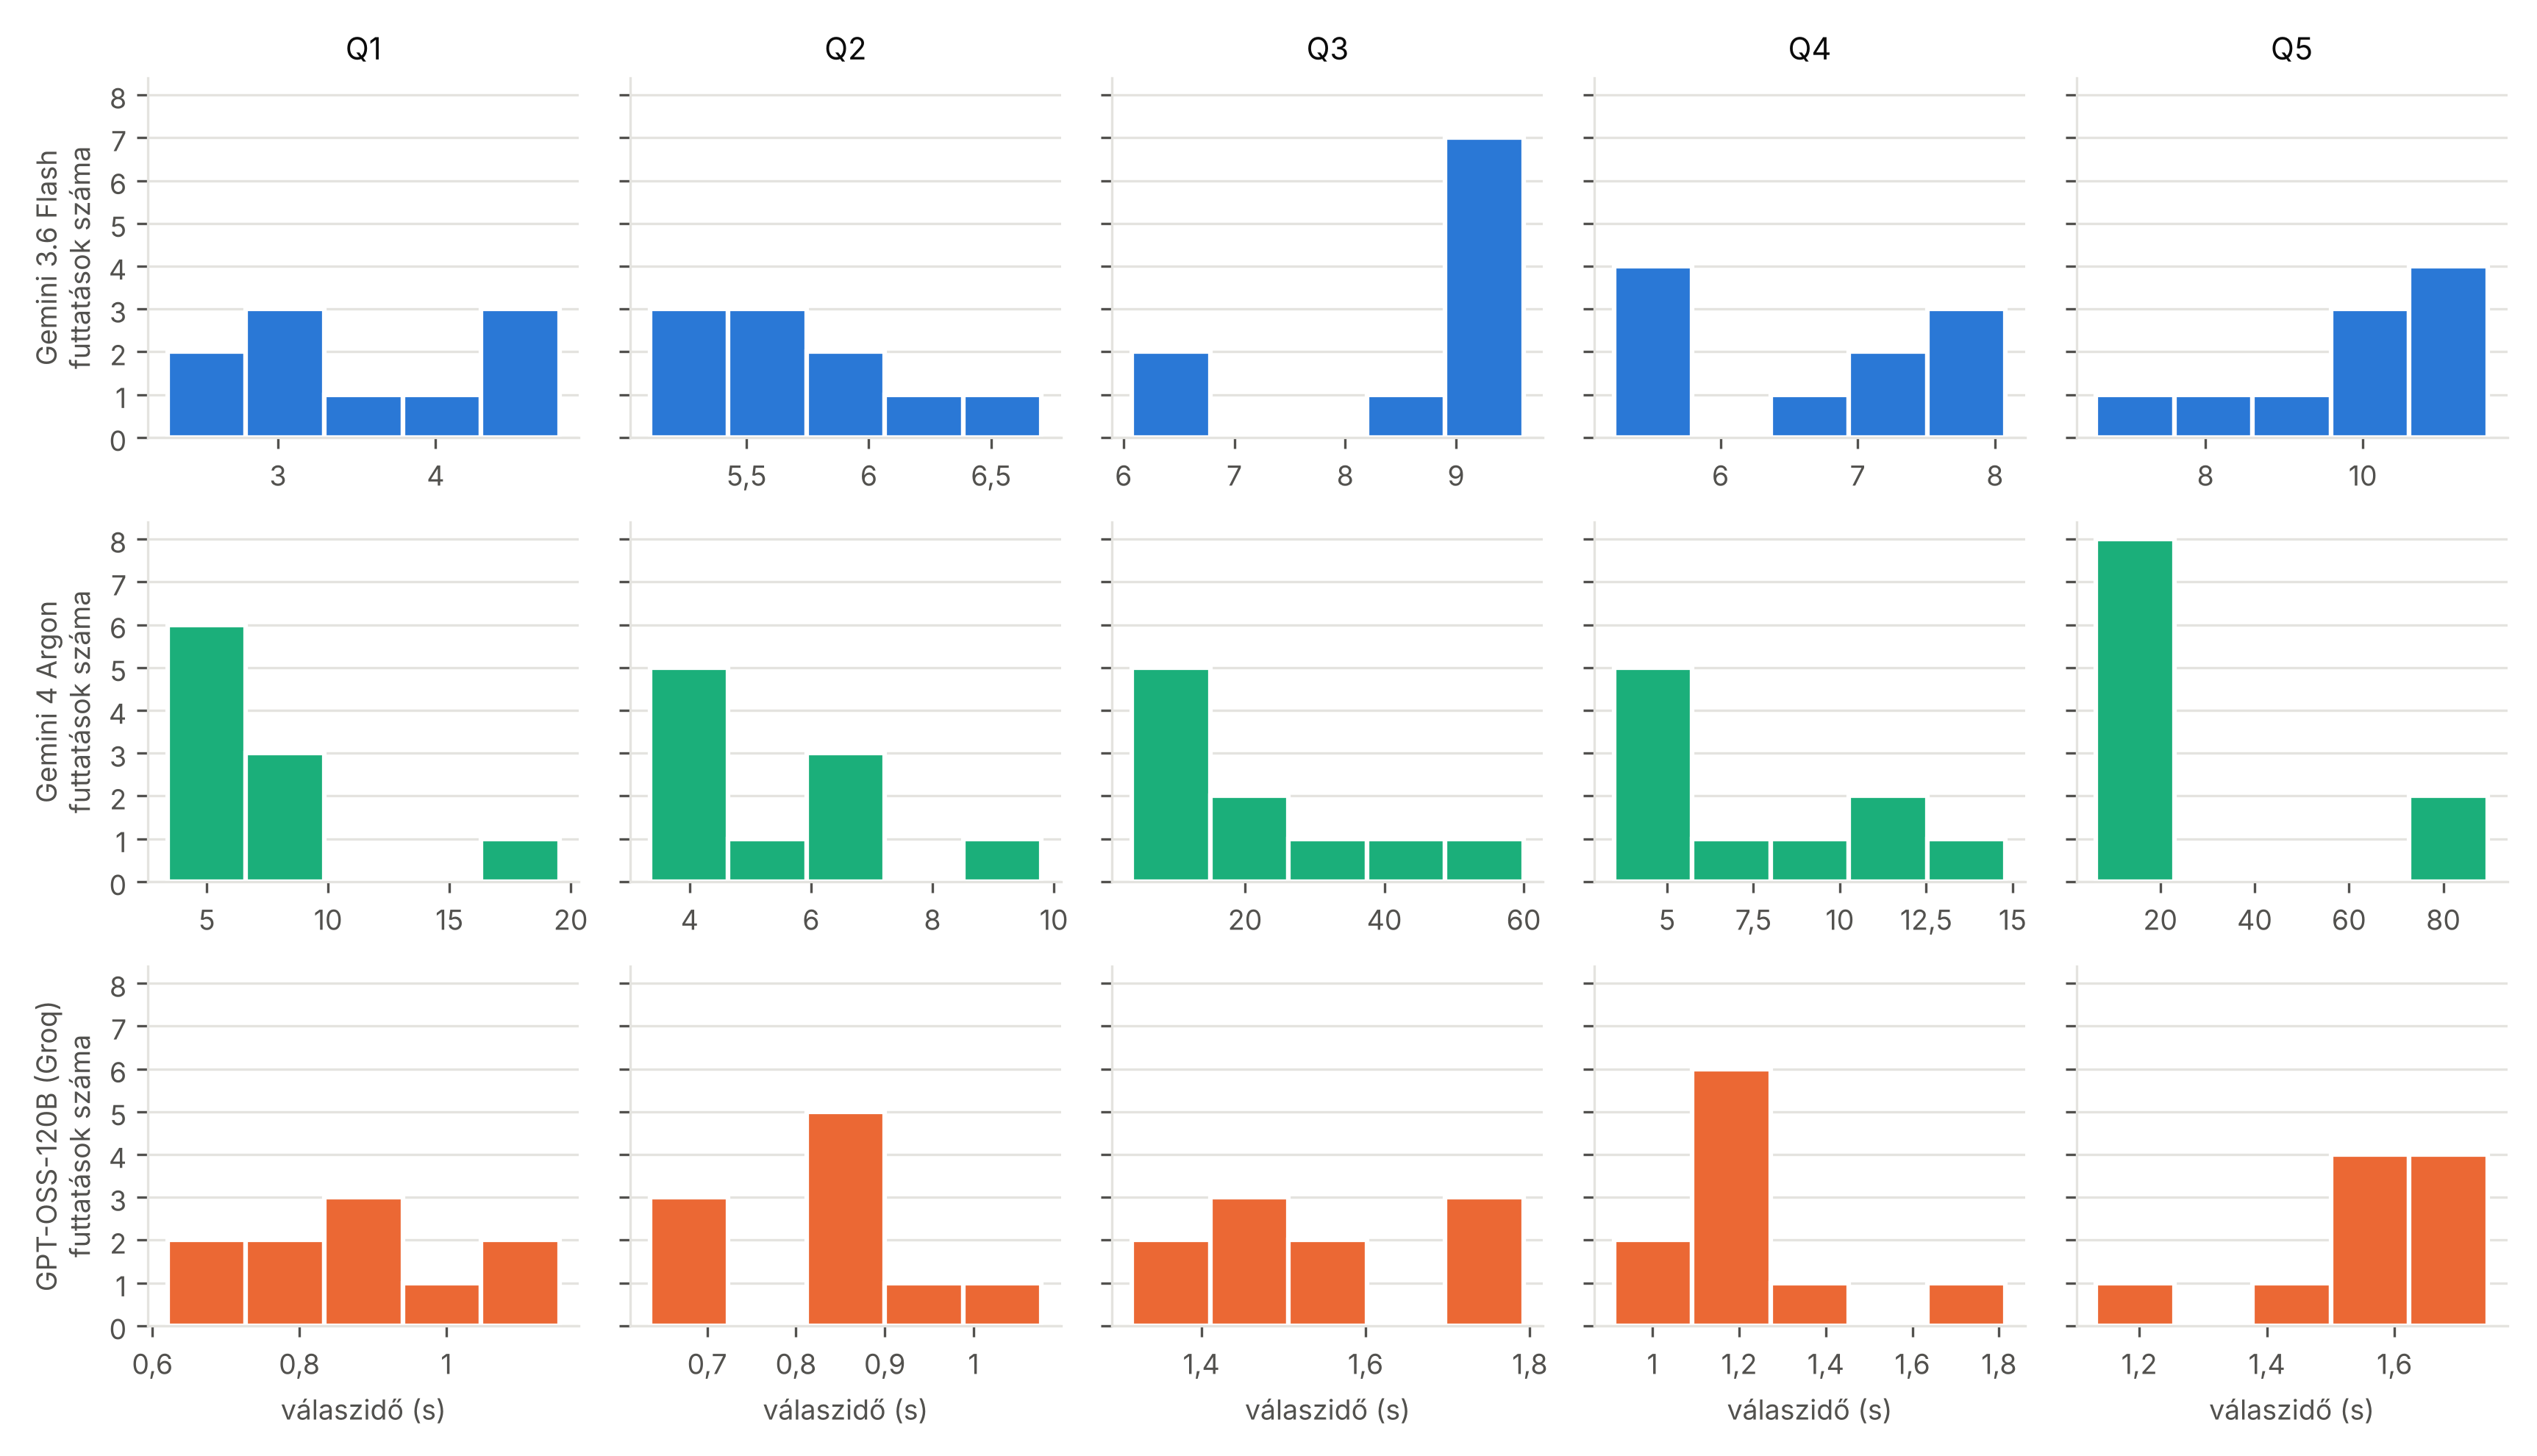
\includegraphics[width=\textwidth]{figures/llm_hist_lekerdezes.png}
	\caption{A válaszidők hisztogramja modellenként és lekérdezésenként. A vízszintes tengelyek skálája panelenként eltér.}
	\label{fig:llm_hist_lekerdezes}
\end{figure}

\begin{figure}[h]
	\centering
	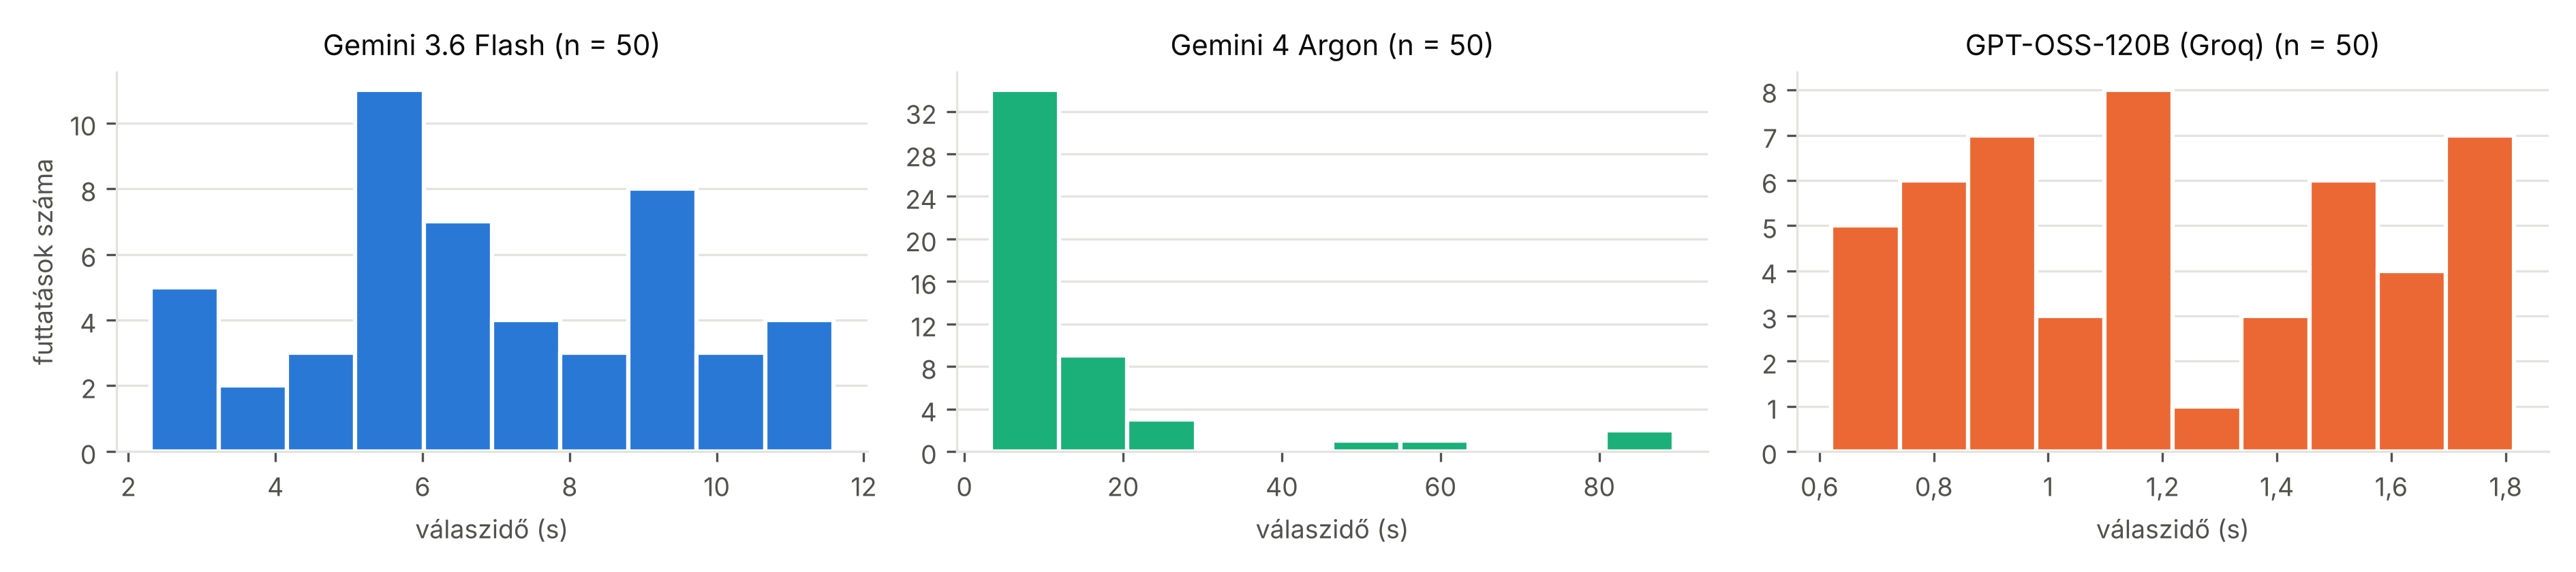
\includegraphics[width=\textwidth]{figures/llm_hist_osszesitett.png}
	\caption{A válaszidők hisztogramja modellenként, az öt lekérdezés összesítve. A vízszintes tengelyek skálája panelenként eltér.}
	\label{fig:llm_hist_osszesitett}
\end{figure}

A mérés költségét \aref{tab:llm-koltseg}. táblázat foglalja össze. A költséget a rögzített tokenszámokból, a szolgáltatók listaárán számoltam. A Gemini modellek a gondolkodási tokeneket kimeneti áron számlázzák. A Gemini 4 Argon az API válaszában nem adta vissza a gondolkodási tokenek számát, ezért az ő költségét a két Gemini modell közös számlázott összegéből számoltam vissza. A Google AI Studio a mérés után 0,31 dollárt mutatott, ebből a Gemini 3.6 Flash pontosan ismert, 0,2193 dolláros részét levonva az Argonra 0,0907 dollár jut. A Groq mérése ingyenes szinten futott, a táblázatban szereplő érték azt mutatja, mennyibe került volna a mérés a fizetős szinten.

\begin{table}[H]
	\centering
	\renewcommand{\arraystretch}{1.3}
	\footnotesize
	\begin{tabular}{|l|r|r|r|r|}
		\hline
		\textbf{Modell} & \textbf{Hívás} & \textbf{Kimeneti token} & \textbf{Összesen} & \textbf{Hívásonként} \\
		& & \textbf{(átlag)} & \textbf{(USD)} & \textbf{(USD)} \\
		\hline
		Gemini 3.6 Flash & 50 & 1152 & 0,2193 & 0,00439 \\
		Gemini 4 Argon & 50 & 159$^{*}$ & 0,0907$^{*}$ & 0,00181$^{*}$ \\
		GPT-OSS-120B (Groq) & 50 & 416 & 0,0136 & 0,00027 \\
		\hline
	\end{tabular}
	\caption{A mérés API-költsége listaáron. A kimeneti tokenek a gondolkodási tokeneket is tartalmazzák. A csillaggal jelölt értékek a számlázott összegből visszaszámolt becslések, a Groq mérése ingyenes szinten futott.}
	\label{tab:llm-koltseg}
\end{table}

\Section{Megfigyelések}

A válaszidők között nagyságrendi különbség mutatkozott. A Groq infrastruktúrán futó GPT-OSS-120B átlagosan 1,2 másodperc alatt válaszolt, és a leglassabb válasza is 2 másodpercen belül megérkezett. A Gemini 3.6 Flash átlaga 6,9, a Gemini 4 Argoné 13,8 másodperc volt. Az Argon mediánja 7,0 másodperc, az átlagot négy kiugróan lassú válasz emeli meg. A Q3 és a Q5 lekérdezésre adott válaszok közül kettő-kettő 47 és 89 másodperc között érkezett meg, miközben ugyanezekre a lekérdezésekre más futtatásokban 4, illetve 6 másodperc alatt is válaszolt. A válaszidő mindhárom modellnél jellemzően a lekérdezés összetettségével nőtt, a leggyorsabb válaszok a Q1 és a Q2, a leglassabbak a Q3 és a Q5 lekérdezésre érkeztek. A válaszidő nagyobb része az első látható token előtt telt el. Ez az arány a Gemini 3.6 Flash esetén átlagosan 95, az Argonnál 89, a GPT-OSS-120B esetén 85 százalék volt, vagyis a válaszidő döntő részét a gondolatmenet és a szerver oldali várakozás teszi ki, nem a kimenet továbbítása.

A két batch eredményei a Gemini modelleknél eltértek egymástól. A Gemini 3.6 Flash mediánja az első batchben 6,1, a másodikban 7,3 másodperc volt, az Argon négy kiugró válaszából három az első, egy a második batchbe esett. A GPT-OSS-120B mediánja mindkét batchben 1,1 másodperc volt. A mintából nem dönthető el, hogy az eltérés a napszaknak vagy a véletlennek tulajdonítható-e, de jól mutatja, hogy a válaszidő egy automatizált pipeline-ban nehezen tervezhető. Ez összhangban van Ouyang és társai \cite{ouyang2025nondeterminism} eredményével, akik szerint a 0 hőmérséklet csökkenti, de nem szünteti meg a kimenetek futtatásonkénti eltérését. A mérés emellett azt is mutatja, hogy az eltérés mértéke modellenként jelentősen különbözik, a nagyobb Gemini 4 Argon kimenete volt a legállandóbb, a gyorsabb és olcsóbb Gemini 3.6 Flash kimenete a legkevésbé.

A kimenetek egyik modellnél sem voltak teljesen állandóak. A legkövetkezetesebbnek a Gemini 4 Argon bizonyult, amely a Q1 és a Q2 lekérdezésre mind a 10 futtatásban ugyanazt a kódot adta, a többi lekérdezésre pedig két változat között váltakozott. A GPT-OSS-120B minden lekérdezésre két változatot adott, ezek egy része csak a \texttt{DbContext} nevében vagy egy záró pontosvesszőben különbözött. A Gemini 3.6 Flash volt a legkevésbé konzisztens. A Q5 lekérdezésre 10 futtatásból 7 eltérő kimenetet adott, és a \texttt{DbContext} változót is négyféleképpen nevezte el (\texttt{context}, \texttt{dbContext}, \texttt{db}, illetve 5 esetben előtag nélkül, csak \texttt{Users} formában). Üres vagy csonka válasz egyik modellnél sem fordult elő.

A változatok többsége ugyanazt az eredményt adja, csak más szerkezetben. A GPT-OSS-120B a Q4 lekérdezésnél a vetítést a rendezés elé tette, a Q5-nél pedig a \texttt{LIKE} feltételt a táblák összekapcsolása előtt alkalmazta. Az Argon a Q5-ben a lapozást a vetítés után végezte. Ezek az átrendezések a relációs műveletek tulajdonságai miatt nem változtatják meg az eredményt. A \texttt{LIKE 'B\%'} mintát a modellek hol \texttt{EF.Functions.Like}, hol \texttt{StartsWith} hívásra képezték le, ugyanazon a modellen belül is futtatásonként változóan. A két alak eredménye a kis- és nagybetűk kezelésében adatbázistól függően eltérhet. A Q3 \texttt{LEFT JOIN} lekérdezésénél a GPT-OSS-120B minden futtatásban, az Argon 3 futtatásban külön kezelte a hiányzó jobb oldali sort, a többi válasz ezt az EF Core SQL-fordítására bízta. Ez Chen és társai \cite{chen2021codex} megfigyelését támasztja alá, miszerint a nyelvi modellek által generált kód helyessége nem garantált, ezért a kimenetet minden esetben ellenőrizni kell.

Egy kimenet hibás volt. A Gemini 3.6 Flash egyik Q3 válaszában az eredményt összeállító lambda egy olyan mezőre (\texttt{x.o}) hivatkozott, amely az adott névtelen típusban nem létezik, így ez a kód le sem fordul. Az előtag nélküli \texttt{Users} formájú válaszok szintén csak akkor fordíthatók, ha a hívó kódban létezik ilyen nevű változó.

A költség szempontjából a gondolkodási tokenek dominálnak. A Gemini 3.6 Flash 50 hívása során 4845 látható és 52\,780 gondolkodási tokent állított elő, így a kimeneti költség 92 százaléka a válaszban meg sem jelenő gondolatmenetre esett. A gondolatmenet hossza a lekérdezés összetettségével nőtt, a Q1 lekérdezésnél átlagosan 415, a Q5-nél 1678 token volt. Ezer lekérdezés fordítása listaáron a Gemini 3.6 Flash esetén körülbelül 4,4, az Argonnál 1,8, a GPT-OSS-120B esetén 0,3 dollárba kerülne. Ezek az összegek kicsik, de minden futtatásnál újra felmerülnek, és a kimenetet utána is ellenőrizni kell.

\Section{Következtetések}

Az LLM-ek interaktív segítségként hasznos eszközök lehetnek, ha egy fejlesztő egyszeri alkalommal szeretne egy SQL lekérdezést LINQ-ra fordítani és az eredményt manuálisan ellenőrzi. A mérésben a legtöbb válasz helyes volt, és a leggyorsabb modell egy másodperc körül válaszolt. Automatizált migrációs pipeline-ban azonban, ahol több száz vagy több ezer lekérdezést kell feldolgozni, a futtatásonként változó kimenet, az előre nem látható válaszidő, az ellenőrizhetőség hiánya és a felhőinfrastruktúra szükségessége komoly akadályt jelent. Már öt rövid lekérdezésen és 150 hívásban is előfordult egy le sem forduló kimenet, és egyik modell sem adott minden lekérdezésre minden futtatásban azonos választ. A determinisztikus fordító ezzel szemben programozottan hívható, az eredménye verifikálható, lokálisan futtatható, és ugyanarra a bemenetre mindig ugyanazt adja.

Az összehasonlítás egy mélyebb architekturális különbséget is feltár, amely a két megközelítés természetéből következik. Az LLM-ek fekete dobozként működnek, azaz a bemenetre adott válasz belső folyamata nem figyelhető meg, nem ellenőrizhető és nem reprodukálható megbízhatóan. Ugyanarra a lekérdezésre a modell más szintaktikai szerkezetet választhat, más segédváltozó-nevet generálhat, és más EF Core metódust alkalmazhat, miközben a kimenetek többnyire szemantikailag egyenértékűek. Ez interaktív, emberi ellenőrzés melletti használatban elfogadható, de automatizált környezetben azt jelenti, hogy a kimenet minden futtatás után felülvizsgálatot igényel.

A determinisztikus fordító ezzel szemben fehér dobozként működik, ahol minden bemeneti tokenhez pontosan meghatározott fordítási szabály tartozik. Az AST csomópontjai egy az egyben megfeleltethetők a generált kód részleteinek, és a teljes fordítási folyamat visszakövethető. Ha a kimenet hibás, a hiba lokalizálható és javítható anélkül, hogy az egész rendszert újra kellene tanítani. Ez az ellenőrizhetőség teszi a determinisztikus fordítót alkalmassá olyan feladatokra, ahol az eredmény helyessége nem opcionális.

\Section{A mérés reprodukálása}

A méréshez használt szkriptek a projekt repójának \texttt{llm\_benchmark} mappájában találhatók. A \texttt{queries.json} a lekérdezéseket, a \texttt{prompt.txt} a prompt sablonját tartalmazza. A \texttt{run\_llm.py} végzi a hívásokat, és minden modell eredményét a \texttt{results} mappa egy-egy \texttt{raw\_<modell>.jsonl} fájljába írja. Az \texttt{analyze.py} ezekből modellenként és lekérdezésenként összesítő statisztikát készít, amelyet a \texttt{results/summary.csv} fájlba ír. A mérés nyers adatai ugyanebben a mappában találhatók. A szkriptekhez Python 3.10 vagy újabb verzió, valamint egy Gemini és egy Groq API kulcs szükséges. A Gemini 4 Argon csak fizetős szinten érhető el. Az alábbi parancsok Windows PowerShellben, az \texttt{llm\_benchmark} mappában futtatandók.

\begin{lstlisting}[language={}]
	py -m venv .venv
	.venv\Scripts\Activate.ps1
	pip install -r requirements.txt
	
	$env:GEMINI_API_KEY = "<Gemini API kulcs>"
	$env:GROQ_API_KEY   = "<Groq API kulcs>"
	
	python run_llm.py --batch-size 5
	python run_llm.py --batch-size 5
	python analyze.py --billed-gemini 0.31
\end{lstlisting}

Az első \texttt{run\_llm.py} hívás lekérdezésenként és modellenként 5 futtatást végez. A második, néhány órával később kiadott hívás a meglévő eredményfájlok alapján csak a hiányzó 5 futtatást pótolja, így a mérés megszakadás esetén is folytatható. A szkript a sikertelen hívásokat, például a kvótahibákat, nem számolja bele a futtatások számába. Az \texttt{analyze.py} \texttt{-{}-billed-gemini} kapcsolója a Gemini projekt számlázott összegét várja, amelyből az Argon költségét számolja. A kapcsoló nélkül a szkript csak a rögzített tokenszámokból számol.

\Chapter{A kódgenerálás deklaratív leírása}
\label{chap:deklarativ}

\Aref{chap:megvalositas}. fejezetben bemutatott fordító a transzformációt és a kódgenerálást is procedurálisan, C\# kódként írja le. A köztes fa csomópontjai a saját kódjukat a \texttt{ToCodeString()} metódusukban maguk állítják elő. Ebben a fejezetben azt vizsgálom, hogyan lehetne a kódgenerálást deklaratívan, a fordító kódjától elkülönülő szabályokkal leírni. Két megközelítést mutatok be, az XSLT alapú transzformációt és a JSON vagy YAML formátumú szabályrendszert. Mindkettő előnye, hogy a célnyelvi szabályok a fordító újrafordítása nélkül módosíthatók.

\Section{XSLT alapú transzformáció}

Az XSLT (Extensible Stylesheet Language Transformations) a W3C által szabványosított, deklaratív nyelv XML dokumentumok átalakítására \cite{w3c1999xslt}. Egy XSLT stíluslap sablonszabályokból áll, amelyek a bemeneti fa csomópontjaira illeszkednek, és meghatározzák, hogy az adott csomópontból milyen kimenet keletkezzen. A kimenet nem csak XML lehet, hanem tetszőleges szöveg is, így az XSLT forráskód generálására is alkalmas.

Ebben a megközelítésben a köztes fát először XML formátumba kellene szerializálni, ahol minden csomóponttípus egy XML elemnek, a csomópont tulajdonságai attribútumoknak, a gyermekcsomópontok pedig beágyazott elemeknek felelnének meg. Az egyes célnyelveket egy-egy stíluslap írná le. \Aref{lst:xslt}. kódpélda egy ilyen stíluslap két sablonszabályát mutatja be, amelyek egy lambda kifejezést és egy tagelérést alakítanak C\# kóddá.

\begin{lstlisting}[language=XML, caption={XSLT sablonszabályok egy lambda kifejezés és egy tagelérés generálására}, label={lst:xslt}]
<xsl:template match="Lambda">
	<xsl:value-of select="@parameter"/>
	<xsl:text> => </xsl:text>
	<xsl:apply-templates select="*"/>
</xsl:template>
	
<xsl:template match="MemberAccess">
	<xsl:apply-templates select="*"/>
	<xsl:text>.</xsl:text>
	<xsl:value-of select="@member"/>
</xsl:template>
\end{lstlisting}

A megközelítés legnagyobb előnye, hogy egy új célnyelv támogatása a fordító újrafordítása nélkül, egy új stíluslap hozzáadásával megoldható. A mintaillesztésen alapuló sablonszabályok természetes módon követik a fa szerkezetét, és a szabvány érettsége miatt az XSLT jól dokumentált, széles körben ismert technológia.

A projekt szempontjából azonban jelentős hátrányai is vannak. A .NET beépített \\ \texttt{XslCompiledTransform} osztálya csak az XSLT 1.0 ajánlást támogatja \cite{mslearn2024xslt}, amely szövegkezelésben és feltételes logikában erősen korlátozott. A kódgenerálás több pontja ráadásul nem írható le egyszerű, csomópontonkénti sablonnal. A \texttt{LEFT JOIN} eredményvetítésének átírása, a skaláris allekérdezések felismerése vagy a dátumfüggvények egységeinek feldolgozása mind olyan döntés, amely a csomópont környezetétől vagy a gyermekekből már előállított kódtól függ. Ezek XSLT 1.0-ban csak nehezen követhető, rekurzív sablonokkal valósíthatók meg. Az átalakítás minden hibája csak futásidőben derülne ki, a stíluslap hibakeresése körülményes, és a köztes fa minden csomóponttípusához XML szerializációt is meg kellene valósítani. A szükséges ráfordítás így a projekt kereteihez képest aránytalanul nagy lett volna.

\Section{Deklaratív szabályrendszer}

Egy másik lehetőség a célnyelvi szabályok JSON vagy YAML formátumú leírása. Egy ilyen szabályrendszer csomóponttípusonként, operátoronként és függvényenként egy-egy helyőrzőket tartalmazó sablont rendelne a célnyelvhez, például a \texttt{SUBSTRING} függvényhez a \\ \texttt{\{0\}.Substring(\{1\} - 1, \{2\})} sablont. Ez a megoldás az egyszerű, egy az egyben megfeleltethető elemeknél (operátorok, skaláris függvények) kényelmes és könnyen bővíthető. A környezetfüggő döntések leírásához viszont a szabályrendszert feltételekkel és saját kifejezésnyelvvel kellene kiegészíteni, ami lényegében egy új sablonnyelv megalkotását jelentené. A megközelítés ezért inkább a procedurális kódgenerálás kiegészítéseként lehet érdekes, például a függvényleképezések külső fájlba szervezésére.

\Section{Összevetés a procedurális leírással}

A két deklaratív megközelítés közös korlátja, hogy a kódgenerálás környezetfüggő döntéseit nehezen fejezik ki. A \texttt{LEFT JOIN} eredményvetítésének átírása vagy a skaláris allekérdezések felismerése olyan döntés, amely nem csak az adott csomóponttól, hanem a környezetétől is függ. Procedurális leírásban ezek egyszerű feltételes utasítások, deklaratív leírásban viszont a szabálynyelv kiterjesztését igénylik. A procedurális leírás további előnye, hogy a hibák nagy részét már a fordítóprogram jelzi, és a meglévő tesztkészlet változtatás nélkül ellenőrzi. Ezért a fordító a procedurális leírásnál maradt, a deklaratív megközelítések pedig egy-egy jól körülhatárolt részfeladatnál, például a függvényleképezések leírásánál jelenthetnek kiegészítést.

\Chapter{Általánosítási és továbbfejlesztési lehetőségek}
\label{chap:altalanositas}

Az előző fejezetekben bemutatott fordító egy kész, tesztelt eszköz, amely SQL utasításokból EF Core kompatibilis LINQ kódot állít elő. A fejlesztés lezárása után felmerült annak a lehetősége, hogy a fordító ne csak egyetlen célnyelvet szolgáljon ki. A grammatika, a parser és a visitor által felépített köztes fa ugyanis nem kötődik szükségszerűen a C\#-hoz, hiszen az SQL lekérdezés szerkezetét írják le. Ha a kódgenerálás cserélhető elemmé válik, ugyanaz a fordító SQL utasításokból tetszőleges célnyelvre képes kódot előállítani, például Java Stream API hívásokra. Ebben a fejezetben az ehhez szükséges átalakítást, a választott megoldást, annak korlátait és a továbbfejlesztés lehetséges irányait mutatom be.

\Section{Motiváció és kiinduló állapot}

Az eredeti tervben a kódgenerálás a köztes fa csomópontjainak feladata volt. Minden csomóponttípus saját \texttt{ToCodeString()} metódussal rendelkezett, amely közvetlenül C\# kódot állított elő. Egy második célnyelv támogatásához tehát első ránézésre elegendő lett volna ezeket a metódusokat egy cserélhető komponensbe kiszervezni.

A kód részletesebb vizsgálata azonban megmutatta, hogy a C\# szintaxis nem csak a csomópontokban, hanem a visitor rétegben is jelen volt. A visitor több helyen kész C\# szöveget írt a köztes fába. Az oszlophivatkozások \texttt{LinqIdentifierNode} csomópontként, stringként összerakott előtagokkal kerültek a fába (\texttt{g.Key}, \texttt{g.FirstOrDefault().Oszlop}, \texttt{x.u.Oszlop}). A szöveg-összefűzés \texttt{string.Concat(...)}, a \texttt{COUNT(DISTINCT ...)} pedig egy teljes \texttt{g.Select(...).Distinct().Count()} kifejezés formájában jelent meg. A \texttt{GETUTCDATE()} és a \texttt{RAND()} függvények eredménye a \texttt{DateTime.UtcNow} és a \texttt{new Random().NextDouble()} szöveg lett, az inline nézetek belső lekérdezése pedig már generált kódként került a fába. Az operátorok (\texttt{==}, \texttt{\&\&}, \texttt{!}) és a \texttt{CAST} céltípusai (\texttt{int}, \texttt{DateTime}) szintén C\# jelölésként szerepeltek. Egy másik célnyelvhez tartozó generátor ezeket a szövegeket már nem tudta volna átalakítani, ezért a kódgenerálás leválasztásához a köztes fát is célnyelv-függetlenné kellett tenni.

\Section{A kódgenerátor interfész}

A cserélhető kódgenerálás megvalósítására a deklaratív leírások mellett egy procedurális lehetőség is kínálkozik. Ebben a megközelítésben a célnyelvi szabályokat egy általános célú programozási nyelven megírt osztály tartalmazza, amely egy rögzített interfészt valósít meg. Ennek előnye, hogy a generátor írója a nyelv teljes kifejezőerejét használhatja, a fordítóprogram ellenőrzi a kódját, és a környezetfüggő döntések is közvetlenül megfogalmazhatók. Hátránya, hogy egy új célnyelv támogatásához programozni kell, és a generátort a fordítóval együtt kell lefordítani. A projekt céljaihoz ez a megközelítés illeszkedik a legjobban, mivel a meglévő \texttt{ToCodeString()} metódusok logikája változtatás nélkül átvihető, és a megoldás a meglévő tesztkészlettel teljes körűen ellenőrizhető.

\Section{Az ICodeGenerator megvalósítása}

Az átalakítás után a fordítás folyamata egy új lépéssel bővült. A visitor továbbra is a köztes fát építi fel, a fából azonban már nem a csomópontok, hanem egy külön kódgenerátor állítja elő a célnyelv kódját. A teljes folyamat tehát a parse fa, a \texttt{SqlVisitor}, a köztes fa, a kódgenerátor és a kimeneti kód láncaként írható le.

A kódgenerátor interfésze a visitor tervezési mintát követi \cite{gamma1994design}. A \\\texttt{ILinqNodeVisitor<T>} interfész a köztes fa minden csomóponttípusához pontosan egy \texttt{Visit} metódust ír elő, összesen harmincat. Az \texttt{ICodeGenerator} ennek a \texttt{string} visszatérési típusú változata, amely a \texttt{Generate} metódussal egy belépési pontot is biztosít. Minden csomópont egy egysoros \texttt{Accept} metódust kapott, amely a generátor megfelelő \texttt{Visit} metódusát hívja meg (\ref{lst:icodegen}. kódpélda).

\begin{lstlisting}[caption={A kódgenerátor interfésze és egy csomópont Accept metódusa}, label={lst:icodegen}]
	public interface ICodeGenerator : ILinqNodeVisitor<string> {
		string Generate(LinqNode root);
	}
	
	public interface ILinqNodeVisitor<out T> {
		T VisitQuery(LinqQueryNode node);
		T VisitMethodCall(LinqMethodCallNode node);
		T VisitLambda(LinqLambdaNode node);
		// ... csomóponttípusonként egy metódus
	}
	
	public class LinqLambdaNode : LinqNode {
		public string ParameterName { get; set; }
		public LinqNode Body { get; set; }
		
		public override T Accept<T>(ILinqNodeVisitor<T> visitor)
		=> visitor.VisitLambda(this);
	}
\end{lstlisting}

A visitor minta választásának több oka is volt. Az interfész maga írja le, hogy egy új generátornak mely csomóponttípusokat kell kezelnie, így az a generátor írójának egyben kitöltendő metóduslistaként is szolgál. Ha a köztes fába új csomóponttípus kerül, minden meglévő generátor fordítási hibát ad mindaddig, amíg az új típus kezelése el nem készül, így egyetlen csomóponttípus kezelése sem maradhat ki észrevétlenül. A minta ráadásul a fordító bemeneti oldalán is jelen van, hiszen az ANTLR által generált \texttt{SqlParserBaseVisitor} szintén erre épül. A fordító így mindkét irányban ugyanazt a bejárási elvet követi.

A C\# kód előállítását a \texttt{CSharpCodeGenerator} osztály végzi, amelybe a korábbi \\ \texttt{ToCodeString()} metódusok logikája változatlan formában került át. A fordító teljes C\# specifikus szintaxisa ebben az egy osztályban található. Az osztály üres sorok és megjegyzések nélkül nagyjából 480 sor, amelynek mintegy harmadát a skaláris SQL függvények leképezése teszi ki. Egy új célnyelvhez tartozó generátor a csomóponttípusok kezelését így nagyjából 200 és 300 sor közötti kóddal valósíthatja meg, amihez a támogatni kívánt függvénykör leképezése adódik hozzá. A \texttt{SqlToLinqConverter} osztály a meglévő hívások mellett egy olyan változatot is kapott, amely paraméterként tetszőleges \texttt{ICodeGenerator} implementációt fogad, generátor megadása nélkül pedig továbbra is a C\# generátort használja.

A köztes fa célnyelv-függetlenné tételéhez a visitor által előállított C\# szövegeket új csomóponttípusok váltották fel. A \texttt{LinqIdentifierNode} megszűnt, helyét a lambda paraméterre hivatkozó \texttt{LinqParameterNode}, a tagelérést leíró \texttt{LinqMemberAccessNode}, valamint a csoportkulcsot \\(\texttt{LinqGroupKeyNode}) és a csoport egy elemét (\texttt{LinqGroupElementNode}) reprezentáló csomópontok vették át. Az operátorok és a \texttt{CAST} céltípusai felsorolás típusként kerülnek a fába, a szöveg-összefűzés és a \texttt{RAND()} a skaláris függvények közös csomópontjára képződik le, a \texttt{COUNT(DISTINCT ...)} pedig az aggregátum csomópont egy jelzőjeként jelenik meg. Az inline nézetek a belső lekérdezés kódja helyett annak részfáját tárolják.

Egy tervezési kérdést tudatosan pragmatikus módon oldottam meg. A köztes fa szerkezete és a metódusnevek (\texttt{Where}, \texttt{Select}, \texttt{OrderBy}, \texttt{GroupBy}) továbbra is a LINQ műveleti modelljét követik, mivel a fordító elsődleges célnyelve a LINQ. Ezek a nevek a fában kanonikus műveletnévként szerepelnek, amelyeket egy másik célnyelv generátora a saját szókészletére fordíthat le. \Aref{lst:javagen}. kódpélda azt mutatja be, hogyan képezhetné le egy Java Stream API-t előállító generátor a metódusneveket.

\begin{lstlisting}[caption={Metódusnevek leképezése egy elképzelt Java Stream generátorban}, label={lst:javagen}]
	public string VisitMethodCall(LinqMethodCallNode node) {
		string name = node.MethodName switch {
			"Where"   => "filter",
			"Select"  => "map",
			"OrderBy" => "sorted",
			"Take"    => "limit",
			"Skip"    => "skip",
			"ToList"  => "toList",
			_ => throw new NotSupportedException(node.MethodName)
		};
		var args = string.Join(", ", node.Arguments.Select(Gen));
		return $".{name}({args})";
	}
\end{lstlisting}

Egy teljesen absztrakt, műveletfajtákat felsorolásként tároló fa a célnyelvektől még függetlenebb lenne, de lényegesen nagyobb átalakítást igényelt volna, és a C\# generátor esetében semmilyen előnnyel nem járt volna.

A fordítás új felépítését \aref{fig:blokk_codegen}. ábra, a kódgenerálásban részt vevő osztályok kapcsolatát \aref{fig:osztaly_codegen}. ábra mutatja.

\begin{figure}[H]
	\centering
	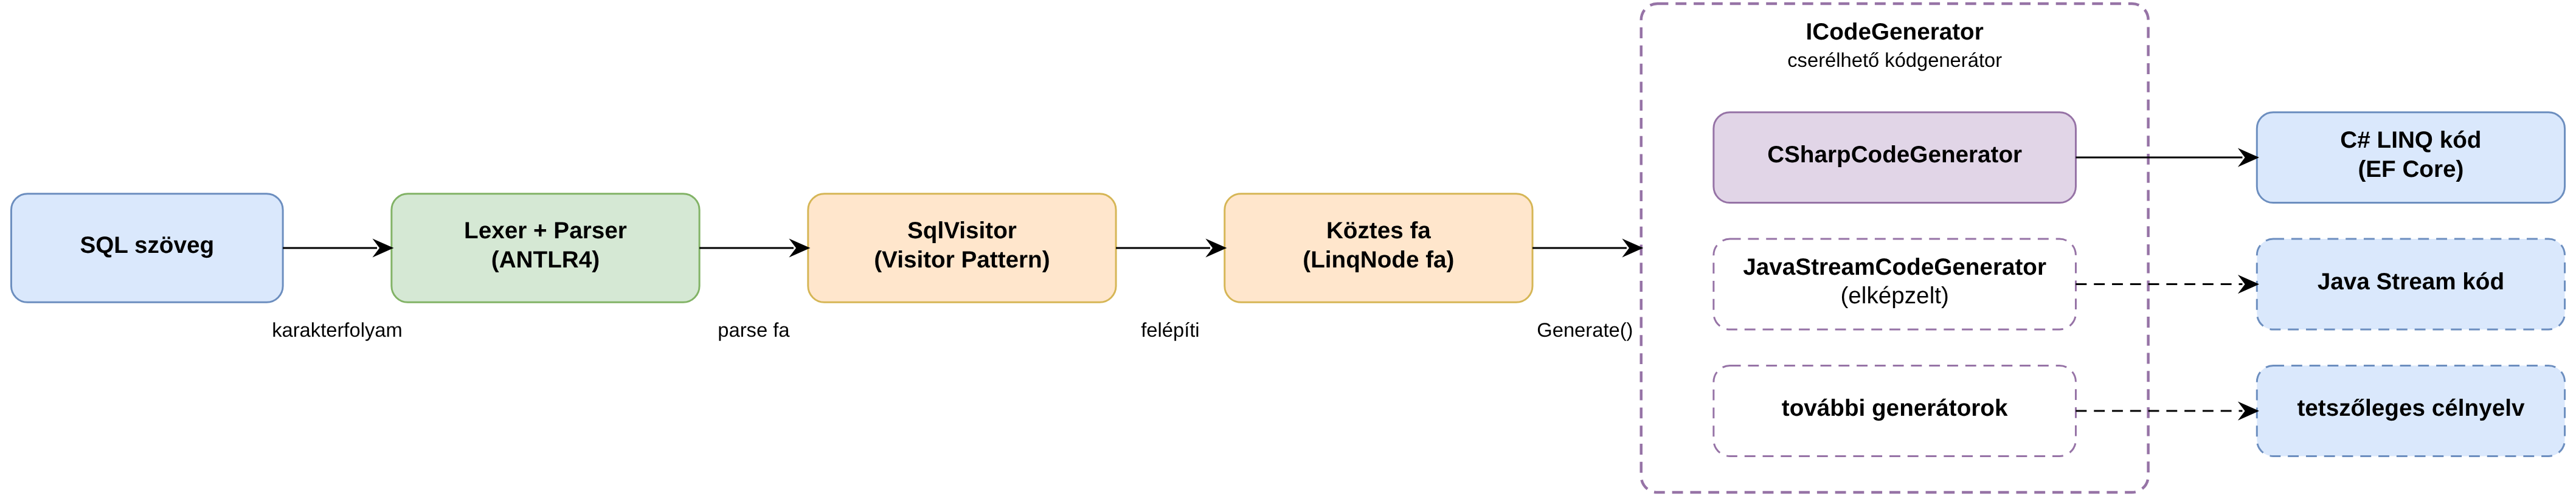
\includegraphics[width=\textwidth]{figures/blokkdiagram_codegen.png}
	\caption{A fordítás folyamata a cserélhető kódgenerátorral}
	\label{fig:blokk_codegen}
\end{figure}

\begin{figure}[H]
	\centering
	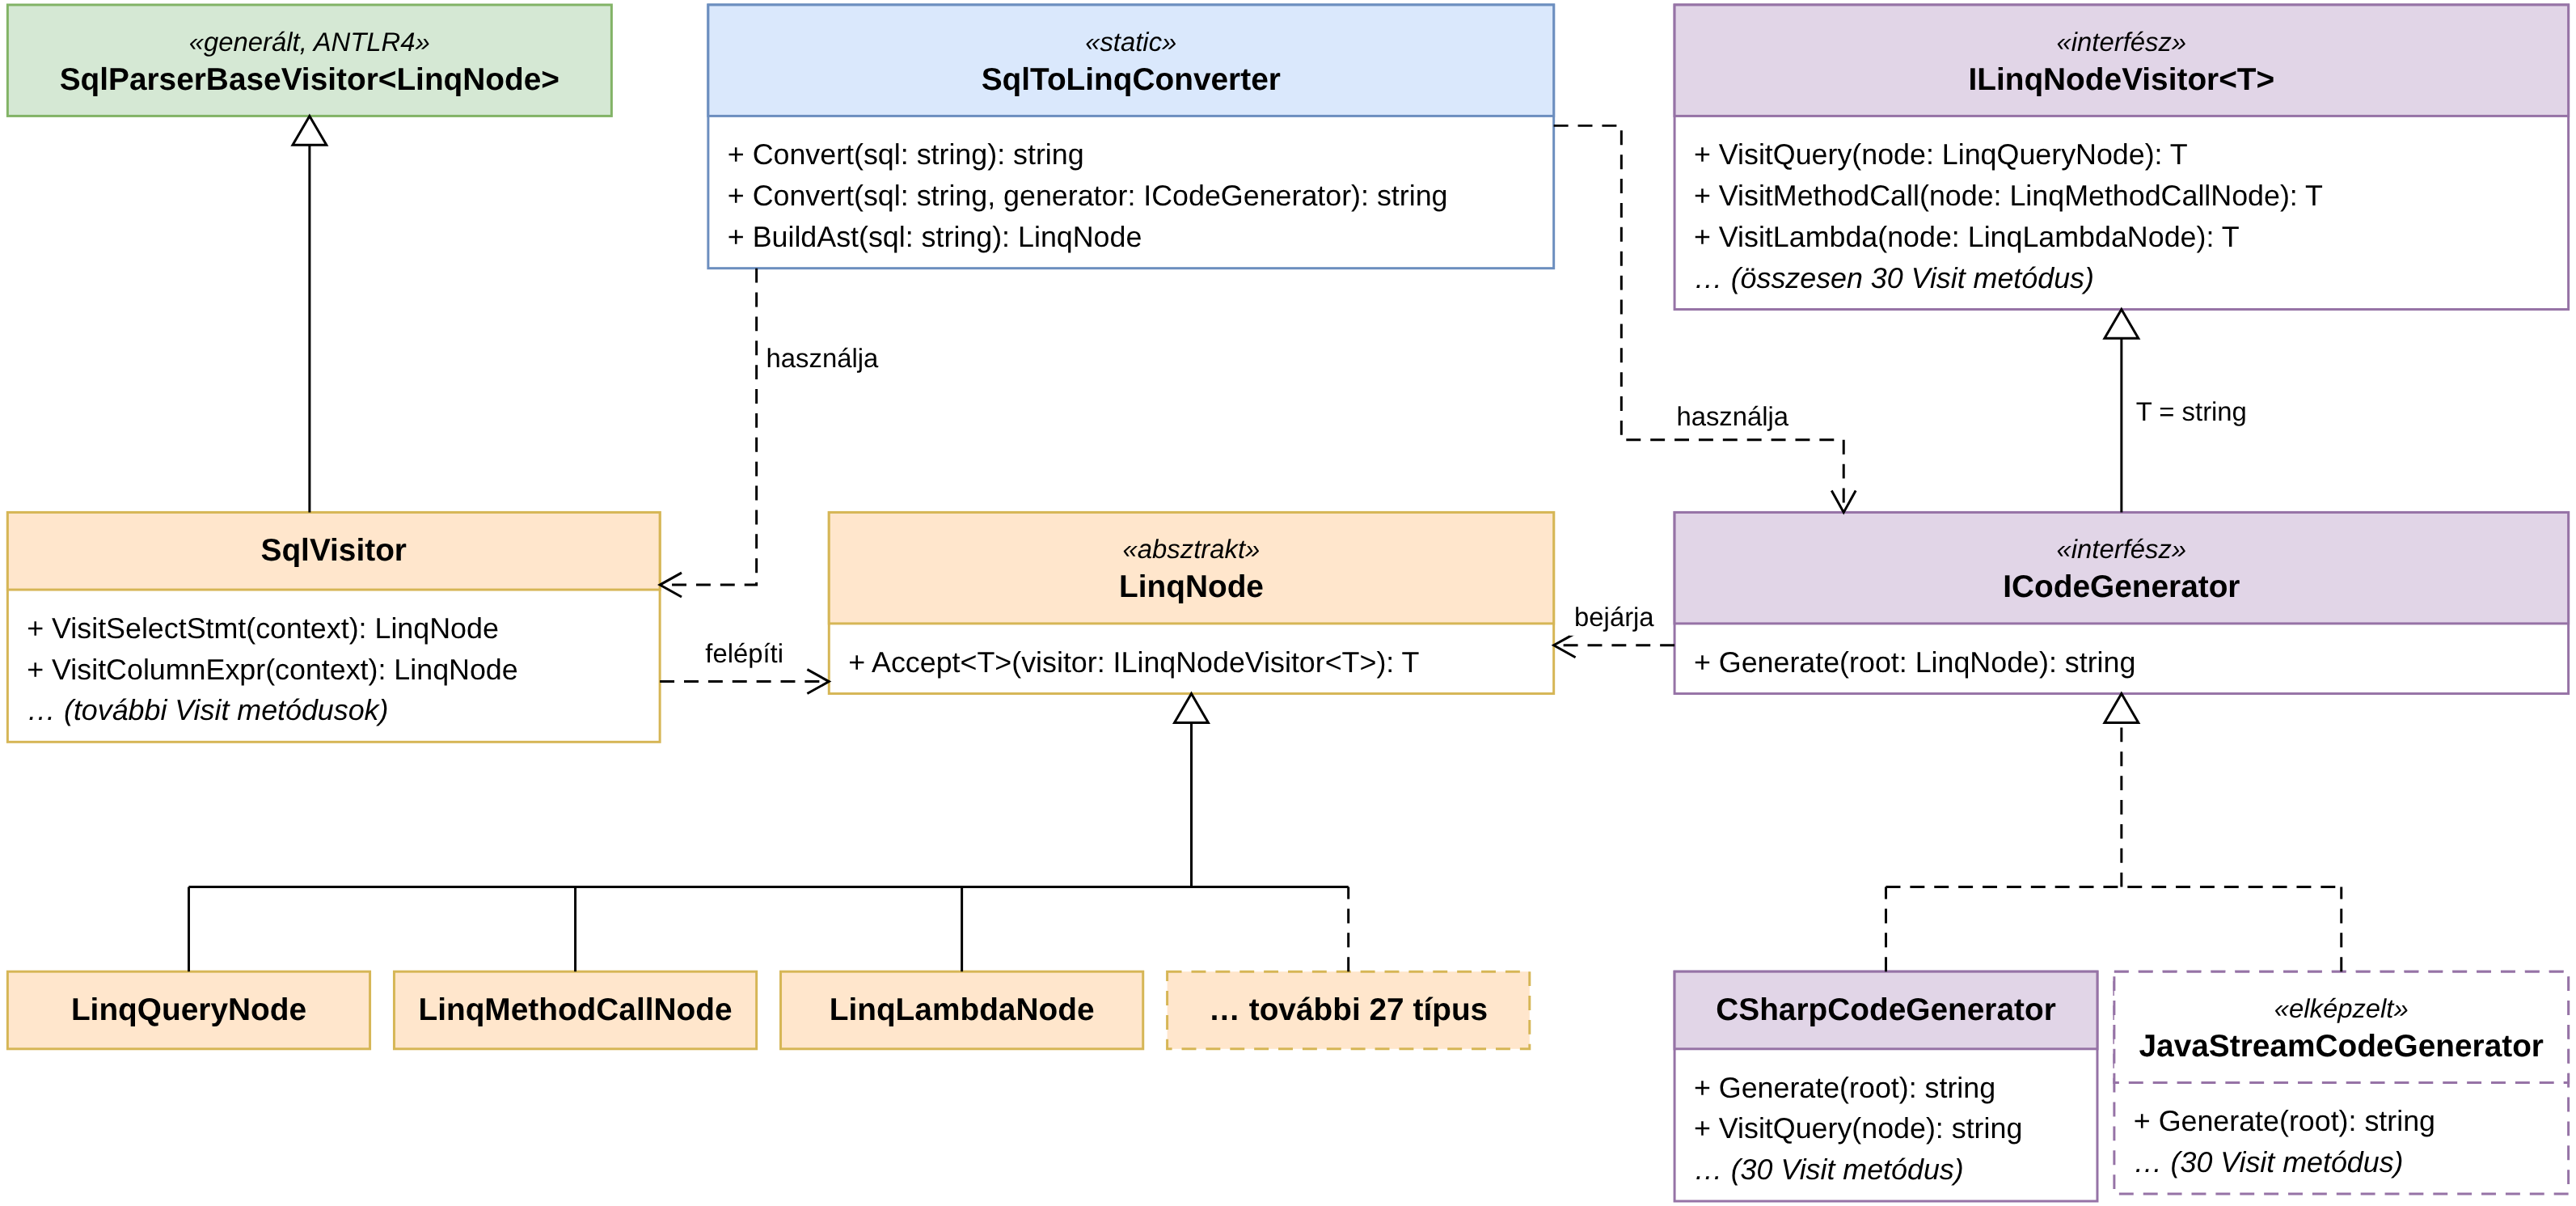
\includegraphics[width=\textwidth]{figures/osztalydiagram_codegen.png}
	\caption{A kódgenerálás osztálydiagramja}
	\label{fig:osztaly_codegen}
\end{figure}

\Section{Az átalakítás ellenőrzése}

Az átalakítás során a fordító viselkedésének változatlannak kellett maradnia. Ennek ellenőrzésére a korábban bemutatott tesztkészlet szolgált. A 267 transpiler teszteset elvárt kimenetén nem kellett módosítani, és az átalakítás után a szemantikai, az EF Core specifikus és a fuzz tesztek is hiba nélkül lefutottak. A string-szintű regressziós tesztek így nem csak a fordító helyességét igazolták, hanem lehetővé tették egy jelentős belső átalakítás biztonságos elvégzését is.

\Section{Korlátok és továbbfejlesztési lehetőségek}

A kódgenerálás leválasztása a szintaktikai különbségeket kezeli, a célnyelvek közötti szemantikai eltéréseket azonban nem. A LINQ és az EF Core legfontosabb tulajdonsága, hogy a lekérdezés kifejezésfaként jut el a providerhez, amely azt SQL-re fordítja és az adatbázisban hajtja végre. A Java Stream API ezzel szemben a memóriában lévő gyűjteményeken dolgozik, így egy Stream alapú generátor kimenete szintaktikailag helyes lehet, a lekérdezés mégis a teljes tábla betöltése után, kliensoldalon futna le. Hasonló eltérés a null-értékek kezelése, mivel a C\# nullable típusai és a \texttt{??} operátor nem minden nyelvben léteznek, a többoszlopos vetítéshez használt névtelen típusok helyett pedig sok nyelvben előre deklarált rekordtípusokra van szükség. A köztes fa LINQ-alakú szerkezete miatt végül egy, a LINQ műveleti modelljétől lényegesen eltérő célnyelv (például egy tisztán deklaratív lekérdezőnyelv) támogatása a fa szerkezetének módosítását is igényelheti. Ezek a kérdések egy konkrét második generátor megvalósításakor válnak eldönthetővé, és további fejlesztési irányt jelölnek ki.
